\documentclass[11pt,a4paper]{article}
\usepackage[utf8]{inputenc}
\usepackage[french]{babel}
\usepackage[T1]{fontenc}
\usepackage{amsmath}
\usepackage{amsfonts}
\usepackage{amssymb}
\usepackage{graphicx}
\usepackage{tikz}
\usepackage[left=2cm,right=2cm,top=2cm,bottom=2cm]{geometry}
\usepackage{hyperref}
\usepackage{float}
\usepackage{xcolor}
\usepackage{pgfplots}
\usepackage{asymptote}
\usepackage[european, straightvoltages, RPvoltages]{circuitikz}
\usetikzlibrary{babel}
\usepackage{siunitx}
\usepackage{wrapfig}
\usepackage{multicol} 
\usepackage{ulem}
\usepackage{listings}
\usepackage{schemabloc}
\usepackage{multicol}
\setlength{\parindent}{0pt}

\title{PROJET EIS - PX222}
\author{Guillemot MOUSSU et Rémi MAZZONE}
\date{2° semestre - 2022-2023}

\definecolor{dkgreen}{rgb}{0,0.6,0}
\definecolor{gray}{rgb}{0.5,0.5,0.5}
\definecolor{mauve}{rgb}{0.58,0,0.82}

\lstset{frame=tb,
language=Python,
aboveskip=3mm,
belowskip=3mm,
showstringspaces=false,
columns=flexible,
basicstyle={\small\ttfamily},
numbers=left,
numberstyle=\tiny\color{gray},
keywordstyle=\color{blue},
commentstyle=\color{dkgreen},
stringstyle=\color{mauve},
breaklines=true,
breakatwhitespace=true,
tabsize=3} 

\begin{document}
\maketitle
\tableofcontents
\listoffigures
\pagebreak

\section{Séance 0 - 21/03/2023}
\subsection{Notes prises au tableau}
\begin{figure} [H]
\begin{center}
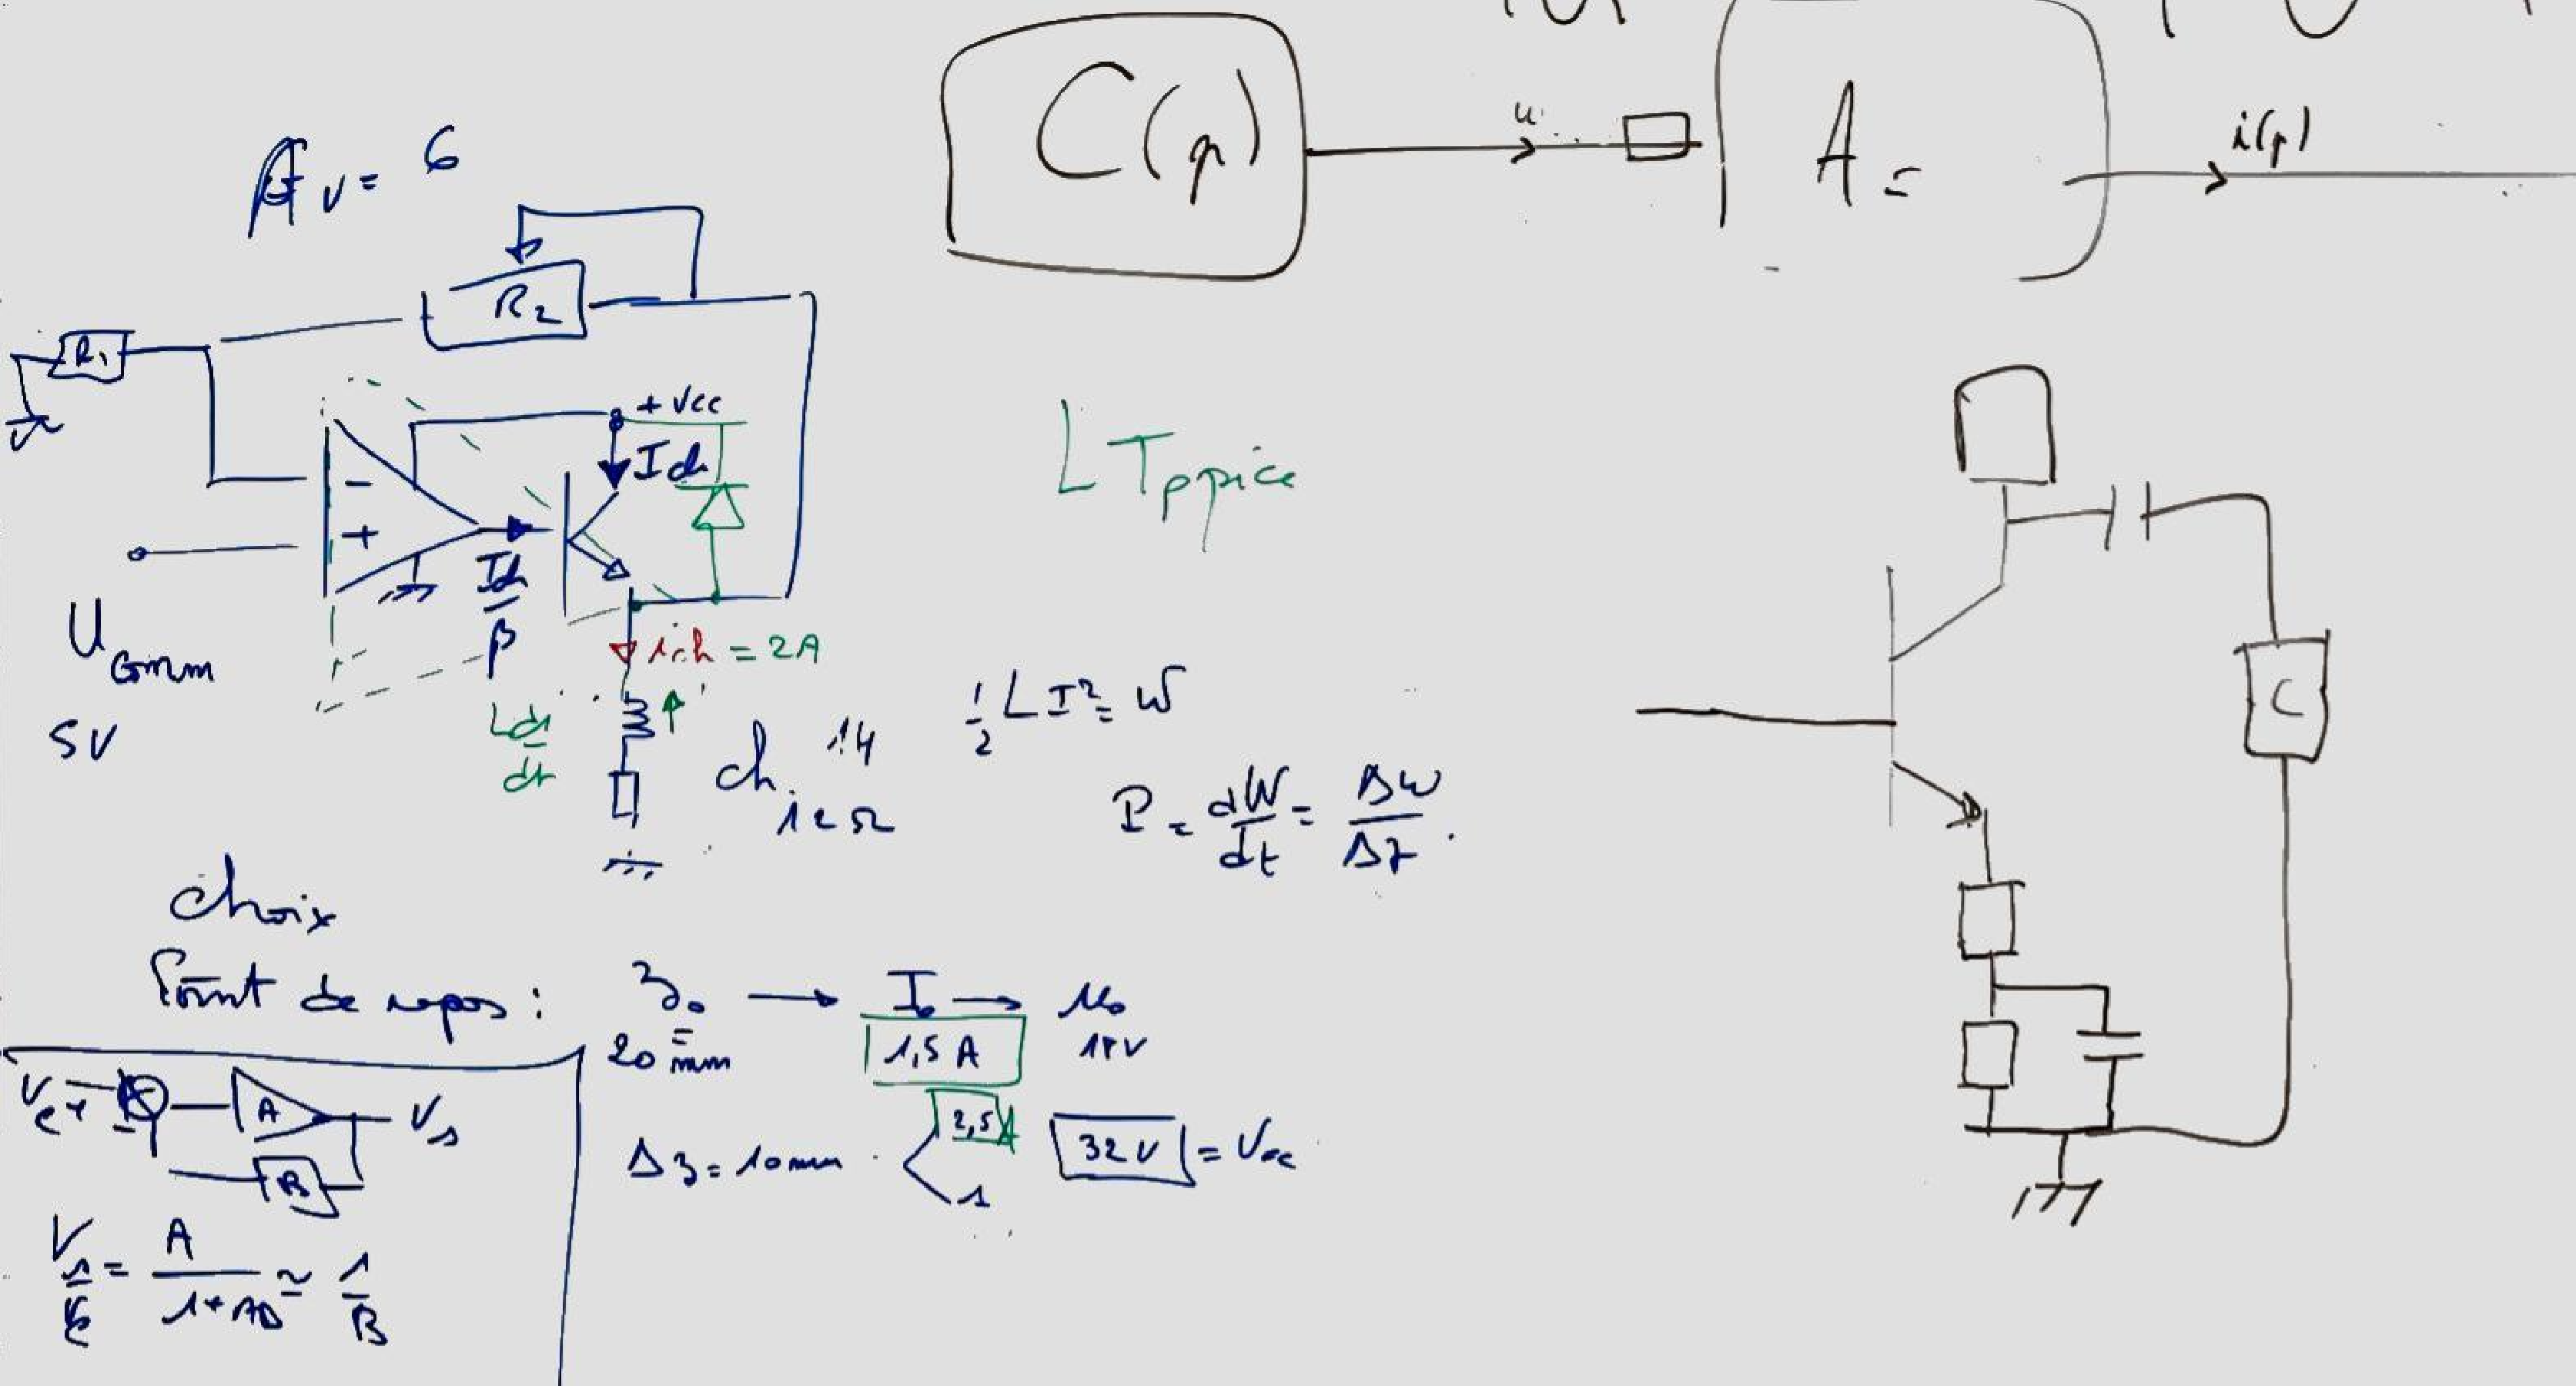
\includegraphics[width=0.9\textwidth]{Schémas/Notes tableau séance 0.png} 
\end{center}
\caption{Notes séance 0}
\end{figure}

\subsection{Idées de plan de recherches}
\begin{itemize}
\item \textbf{Caractérisation de la bobine} : mesure de la résistance et l'inductance de la bobine. Cela permettra de modéliser la bobine et de calculer le champ magnétique qu'elle produit
\item \textbf{Modélisation de la bobine} : utilisation des valeurs mesurées pour construire un modèle électrique de la bobine, par exemple en utilisant l'équation de l'inductance d'une bobine. Pour une précision plus élevée, il peut être nécessaire d'inclure d'autres effets tels que la saturation du noyau de la bobine ou la résistance série équivalente
\item \textbf{Étude du champ magnétique de la bobine} : calcul de la distribution du champ magnétique à l'aide d'un logiciel de simulation. Validation des résultats expérimentalement
\item \textbf{Choix d'un capteur de distance} : choix d'un capteur de distance infrarouge adapté à la plage de mesure et à la précision requises. La fréquence de mesure et la plage de mesure peuvent influencer le résultat
\item \textbf{Calibration du capteur de distance} : déterminer la relation entre la tension de sortie du capteur et la distance de la bille par rapport à la bobine
\item \textbf{Conception d'un correcteur } : utiliser les données obtenues précédemment pour concevoir un correcteur proportionnel-intégral-dérivé (PID) ou un correcteur à avance de phase pour contrôler la position de la bille. C'est la partie clé de ce projet. Le correcteur PID est une méthode de contrôle classique qui est souvent utilisée pour les systèmes de positionnement. Un correcteur à avance de phase peut également être utilisé pour améliorer les performances.
\item \textbf{Implémentation du correcteur } : test du correcteur via Matlab et Simulink
\item \textbf{Étalonnage du système} : ajuster les paramètres du correcteur pour atteindre la précision et la stabilité requises
\item \textbf{Validation du système} : tester le système dans différentes conditions et valider ses performances
\item \textbf{Optimisation du système} : améliorer le système en optimisant les paramètres du correcteur et en utilisant des techniques avancées de contrôle, telles que le contrôle prédictif et le contrôle adaptatif
\end{itemize}
\medskip
Il est important de noter que certains des points ont déjà été réalisés lors du premier semestre

\pagebreak
\section{Séance 1 - 05/04/2023}
\subsection{Reprise des éléments du semestre précédent}
Avec Hopkinson, nous avions obtenu un schéma équivalent de la bobine : 
\begin{figure}[H]
\begin{center}
\begin{circuitikz}
\draw
(0,0) to [V=$\varepsilon$] (0,2)
(0,2) to [short, i=$\varphi$] (2,2)
(2,2) to [R, l=$\mathfrak{R}_1$] (2,0)
(2,0) to [short] (0,0)
(2,2) to [R, l=$\mathfrak{R}(z)$, *-] (5,2)
(2,0) to [R, l=$\mathfrak{R}_0$, *-] (5,0)
(5,2) to [short] (5,0);
\end{circuitikz}
\caption{Modélisation de la bobine}
\end{center}
\end{figure}

Nous avions trouvé que la fonction de transfert de la bobine est : $\boxed{T_{BO}=\dfrac{Z}{I}=\dfrac{k_i}{k_z-mp^2}}$\\
Avec les valeurs suivantes :\\
\medskip
$I_0 = 2A$, $Z_0 = 22mm$, $L_1 = 6.73H$, $\alpha = 2.06$, $m = 35.8g$\\
$k_i = \dfrac{I_0 \cdot L_1 \cdot \alpha}{(1 + \alpha \cdot Z_0)^2}$, $k_z = \dfrac{I_0^2 \cdot L_1 \cdot \alpha^2}{(1 + \alpha \cdot Z_0)^3}$

\subsection{Utilisation de Matlab}
\label{Matlab1}
Nous avons donc notre fonction de transfert. Une idée qui nous est venue est d'adapter les scripts pour utiliser l'outil de M. Mendes que nous avons découvert en TP. Cela devrait nous permettre de calculer notre correcteur. Pour commencer, on a placé nos valeurs dans Matlab et tracé le bode obtenu. Cette étape est présente seulement pour nous faire une idée du système à l'heure actuelle

\begin{figure}[H]
Code Matlab que nous avons utilisé :
\begin{lstlisting}[language=Matlab]
I0 = 2;
Z0 = 22 * 10^-3;
L1 = 6.73;
alpha = 2.06;
ki = (I0 * L1 * alpha) / (1 + alpha * Z0) ^2;
kz = -(I0 ^2 * L1 * alpha ^2) / (1 + alpha * Z0) ^3;
m = 35.8;

num =  ki ;
den = [(-m) 0 kz];
sys = tf(num,den);

figure;
bode(sys)
grid on
figure;
nyquist(sys)
grid on
\end{lstlisting}
\end{figure}

\pagebreak
On obtient donc le bode suivant :
\begin{figure} [H]
\begin{center}
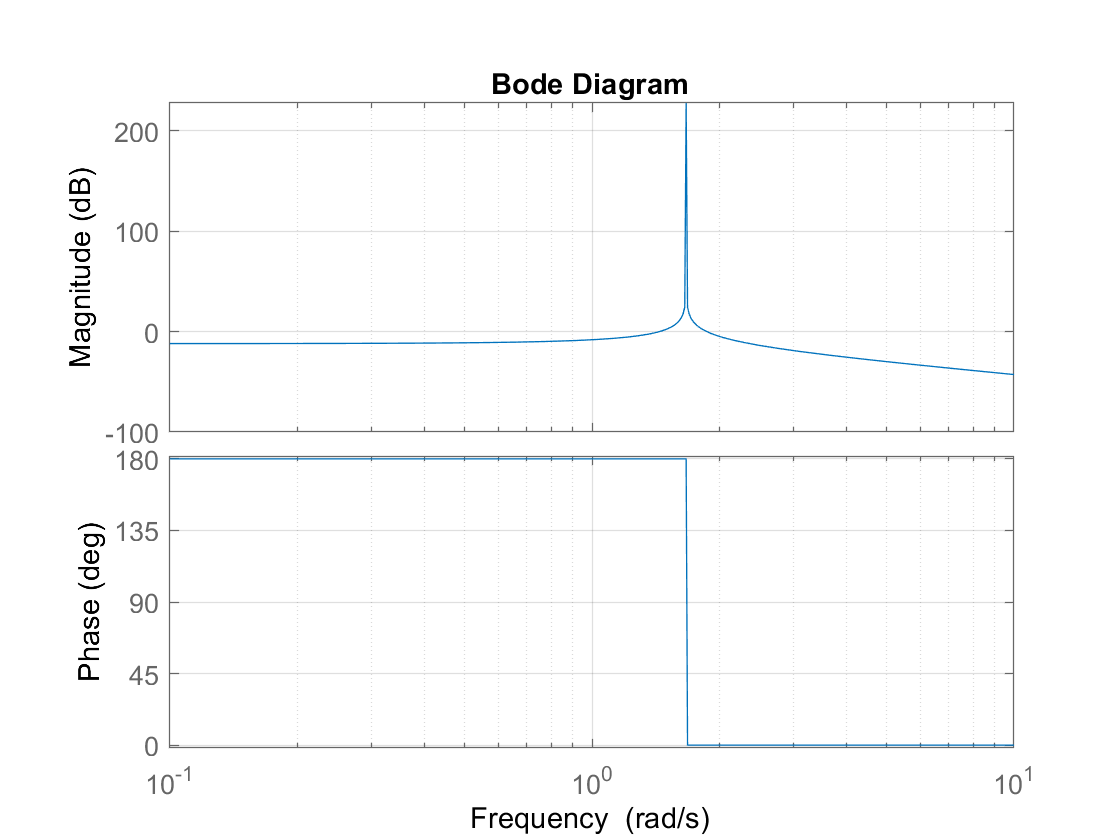
\includegraphics[width=0.9\textwidth]{Schémas/Bode initial.png} 
\end{center}
\caption{Bode obtenu}
\label{fig:Bode initial}
\end{figure}

On trace ensuite le diagramme de Nyquist :
\begin{figure} [H]
\begin{center}
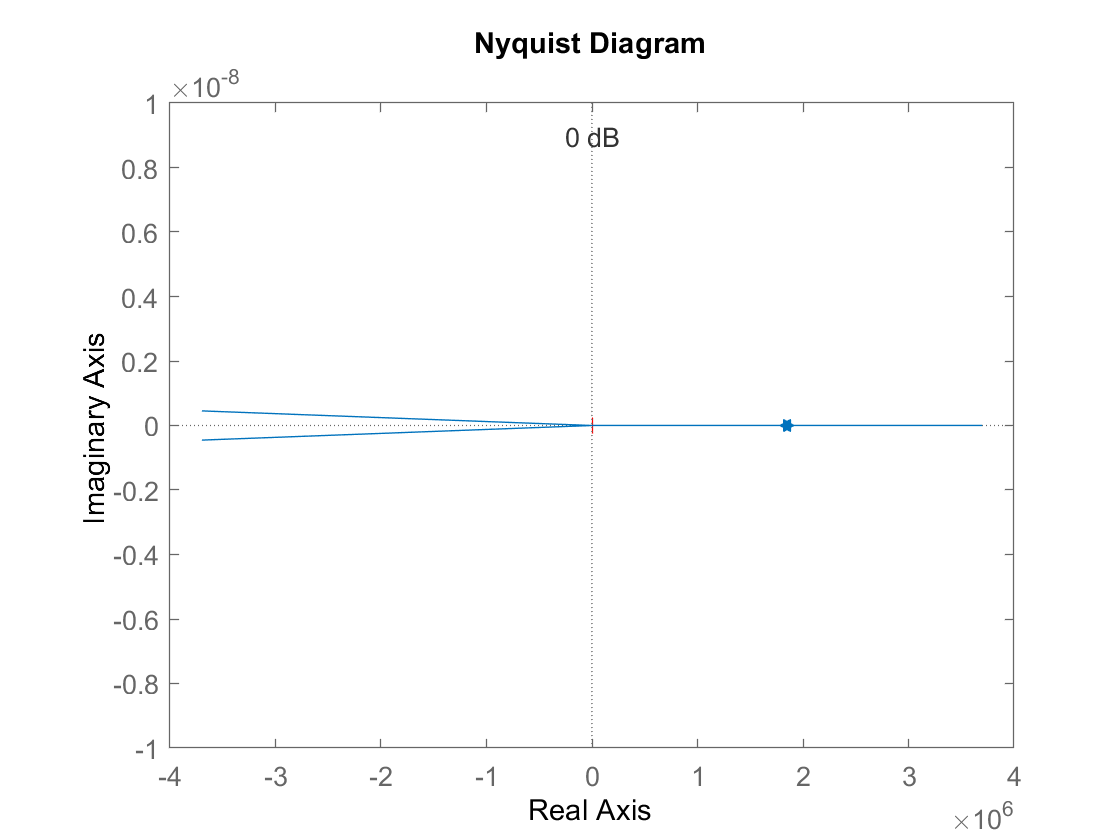
\includegraphics[width=0.6\textwidth]{Schémas/Nyquist initial.png} 
\end{center}
\caption{Nyquist obtenu}
\label{fig:Nyquist initial}
\end{figure}

On remarque donc qu'il reste du travail avant d'avoir un résultat satisfaisant, mais nous reviendrons sur ce point ultérieurement

\subsection{Modélisation point par point du système}
\label{Modélisation point par point}
L'objectif est de réaliser un circuit correspondant à ce schéma bloc :

\begin{figure} [H]
\begin{center}
\begin{tikzpicture}
\sbEntree{E}
\sbSumb{comp}{E}                
\sbRelier[$C$]{E}{comp}
\sbBloc{reg}{$R$}{comp}  
\sbRelier[$\varepsilon$]{comp}{reg}
\sbBloc{amp}{$A$}{reg}
\sbRelier[$U$]{reg}{amp}
\sbBloc{sys}{$H$}{amp}      
\sbRelier[$X$]{amp}{sys}
\sbSortie{S}{sys}                
\sbRelier[$Y$]{sys}{S}
\sbDecaleNoeudy[4]{S}{U}
\sbBlocr{cap}{$B$}{U}        
\sbRelieryx{sys-S}{cap}
\sbRelierxy[$Y_m$]{cap}{comp}
\end{tikzpicture}
\end{center}
\caption{Schéma bloc du système}
\label{fig:Schéma bloc}
\end{figure}

\subsubsection{Modélisation de l'amplificateur}
\label{Modélisation ampli}
Nous avons en sortie d'un STM8 un signal de 5V, nous voulons que la bobine soit alimentée en 30V. Pour cela on utilise un amplificateur à AOP, en série avec un transistor bipolaire. On a le schéma classique d'un amplificateur à AOP :

\begin{figure} [H]
\begin{center}
\begin{tikzpicture}
% Schéma bloc
\sbEntree{E}
\sbBloc{amp}{$A$}{E}
\sbRelier[$U$]{E}{amp}
\sbSortie{S}{amp}
\sbRelier[$X$]{amp}{S}

% Flèche entre les deux schémas
\draw[->, thick] (4,0) -- (6,0);

% Schéma elec
\draw (11,0) node[op amp] (opamp) {};
\draw (opamp.-) to[R, l=$R_1$] ++(-2,0) node[ground] {};
\draw (opamp.+) to[short, -*] ++(-0.5,0) node[label=left:$U$] {};
\draw (opamp.-) to[short] ++(0,1) coordinate (feedback);
\draw (feedback) to[R, l=$R_2$] ++(2,0) -| (opamp.out);
\draw (opamp.out) to[short, -o] ++(1,0) node[label=right:$X$] {};
\end{tikzpicture}
\end{center}
\caption{Amplificateur à AOP}
\label{fig:Amplificateur à AOP}
\end{figure}

Si on ajoute le transistor et la bobine au schéma, cela nous donne :
\begin{figure} [H]
\begin{center}
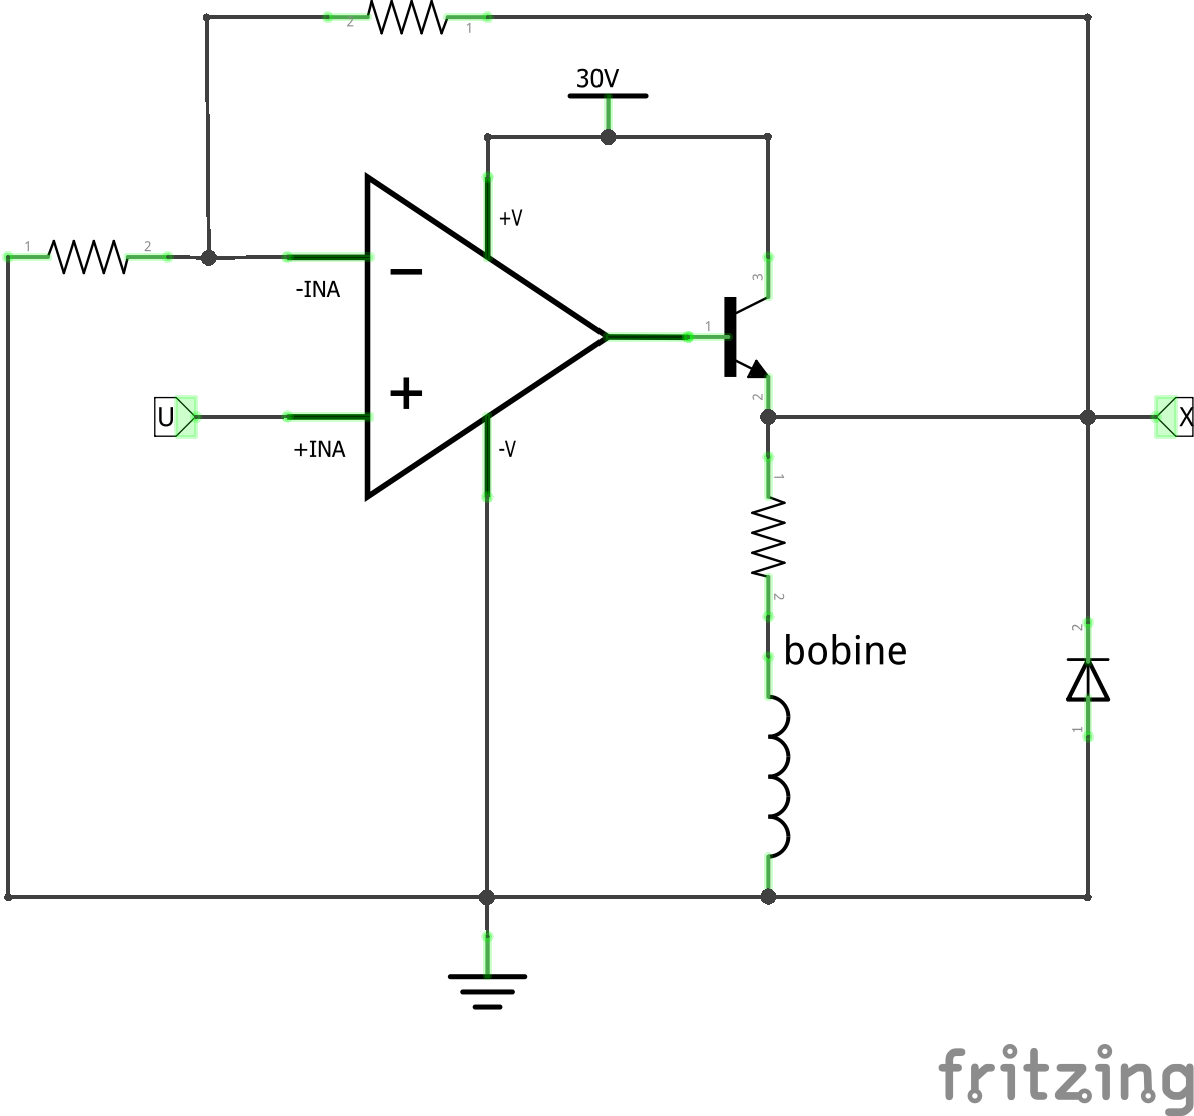
\includegraphics[width=0.6\textwidth]{Schémas/Ampli.png} 
\end{center}
\caption{Modélisation du bloc amplificateur}
\label{fig:Modélisation du bloc amplificateur}
\end{figure}

\subsubsection{Modélisation d'un régulateur PD}
\label{Modélisation PD}
On a le schéma classique d'un régulateur PD :

\begin{figure} [H]
\begin{center}
\begin{tikzpicture}
% Schéma bloc
\sbEntree{E}
\sbBloc{amp}{$R$}{E}
\sbRelier[$\varepsilon$]{E}{amp}
\sbSortie{S}{amp}
\sbRelier[$U$]{amp}{S}

% Flèche entre les deux schémas
\draw[->, thick] (4,0) -- (6,0);

% Schéma elec
\draw (11,0) node[op amp] (opamp) {};
\draw (opamp.-) to[R, l=$R_1$] ++(-2,0) coordinate (entry) {};
\draw (entry) to [short, -o] ++(-0.5,0) node[label=left:$\varepsilon$] {};
\draw (entry) to[short] ++(0,1) coordinate (pointC);
\draw (pointC) to [C, l=$C$] ++(2,0) -| (opamp.-);
\draw (opamp.+) to[short, -] ++(-0.5,0) node[ground] {};
\draw (opamp.-) to[short] ++(0,1) coordinate (feedback);
\draw (feedback) to[R, l=$R_2$] ++(2,0) -| (opamp.out);
\draw (opamp.out) to[short, -o] ++(1,0) node[label=right:$U$] {};
\end{tikzpicture}
\end{center}
\caption{Régulateur PD}
\label{fig:Régulateur PD}
\end{figure}

Si on donne le schéma complet de ce bloc, cela nous donne :

\begin{figure} [H]
\begin{center}
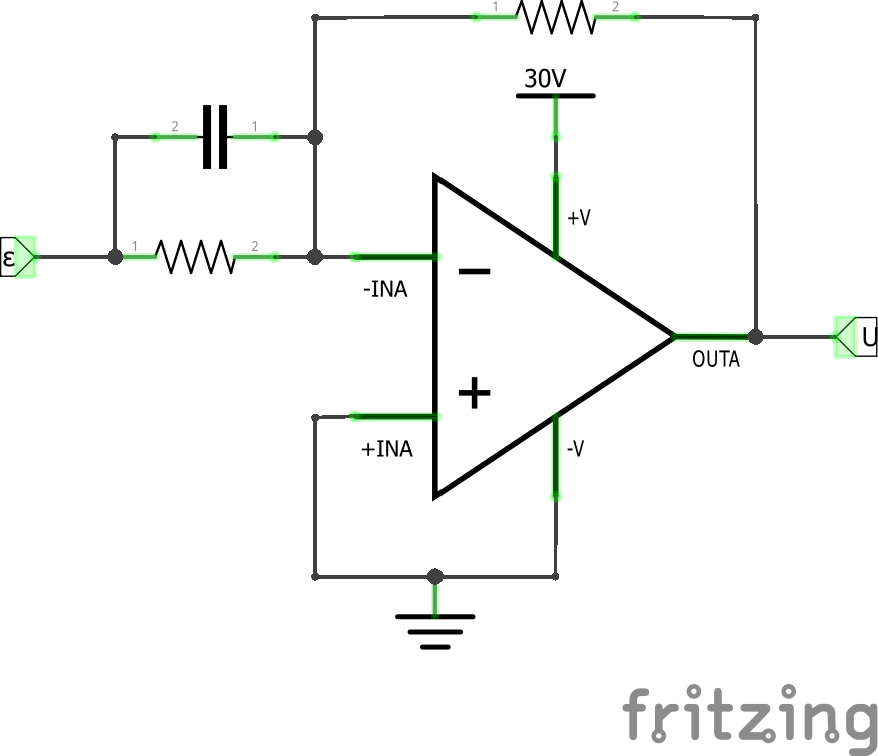
\includegraphics[width=0.5\textwidth]{Schémas/Correcteur PD.png} 
\end{center}
\caption{Modélisation du bloc régulateur (PD)}
\label{fig:Modélisation du bloc régulateur (PD)}
\end{figure}

\subsubsection{Modélisation d'un régulateur PID}
\label{Modélisation PID}
Dans le cas où l'on souhaite finalement modéliser un régulateur PID, on doit ajouter un condensateur en parallèle de notre résistance :

\begin{figure} [H]
\begin{center}
\begin{circuitikz}
\draw (0,0) node[op amp] (opamp) {};
\draw (opamp.-) to[R, l=$R_1$] ++(-2,0) coordinate (entry) {};
\draw (entry) to [short, -o] ++(-0.5,0) node[label=left:$\varepsilon$] {};
\draw (entry) to[short] ++(0,1) coordinate (pointC);
\draw (pointC) to [C, l=$C_1$] ++(2,0) -| (opamp.-);
\draw (opamp.+) to[short, -] ++(-0.5,0) node[ground] {};
\draw (opamp.-) to[short] ++(0,1) coordinate (feedback);
\draw (opamp.-) to[short] ++(0,2.5) coordinate (feedback2);
\draw (feedback) to[R, l=$R_2$] ++(2,0) -| (opamp.out);
\draw (feedback2) to[C, l=$C_2$] ++(2,0) -| (opamp.out);
\draw (opamp.out) to[short, -o] ++(1,0) node[label=right:$U$] {};
\end{circuitikz}
\end{center}
\caption{Régulateur PID}
\label{fig:Régulateur PID}
\end{figure}

\subsubsection{Modélisation du système complet (PD)}
\label{Modélisation complète}
On choisit le régulateur PD pour représenter le système complet. On a vu qu'il suffira d'ajouter une capacité pour passer à un régulateur PID au besoin. On repère bien les blocs comparateur, amplificateur (A), régulateur (R) et capteur (B)

\begin{figure} [H]a	
\begin{center}
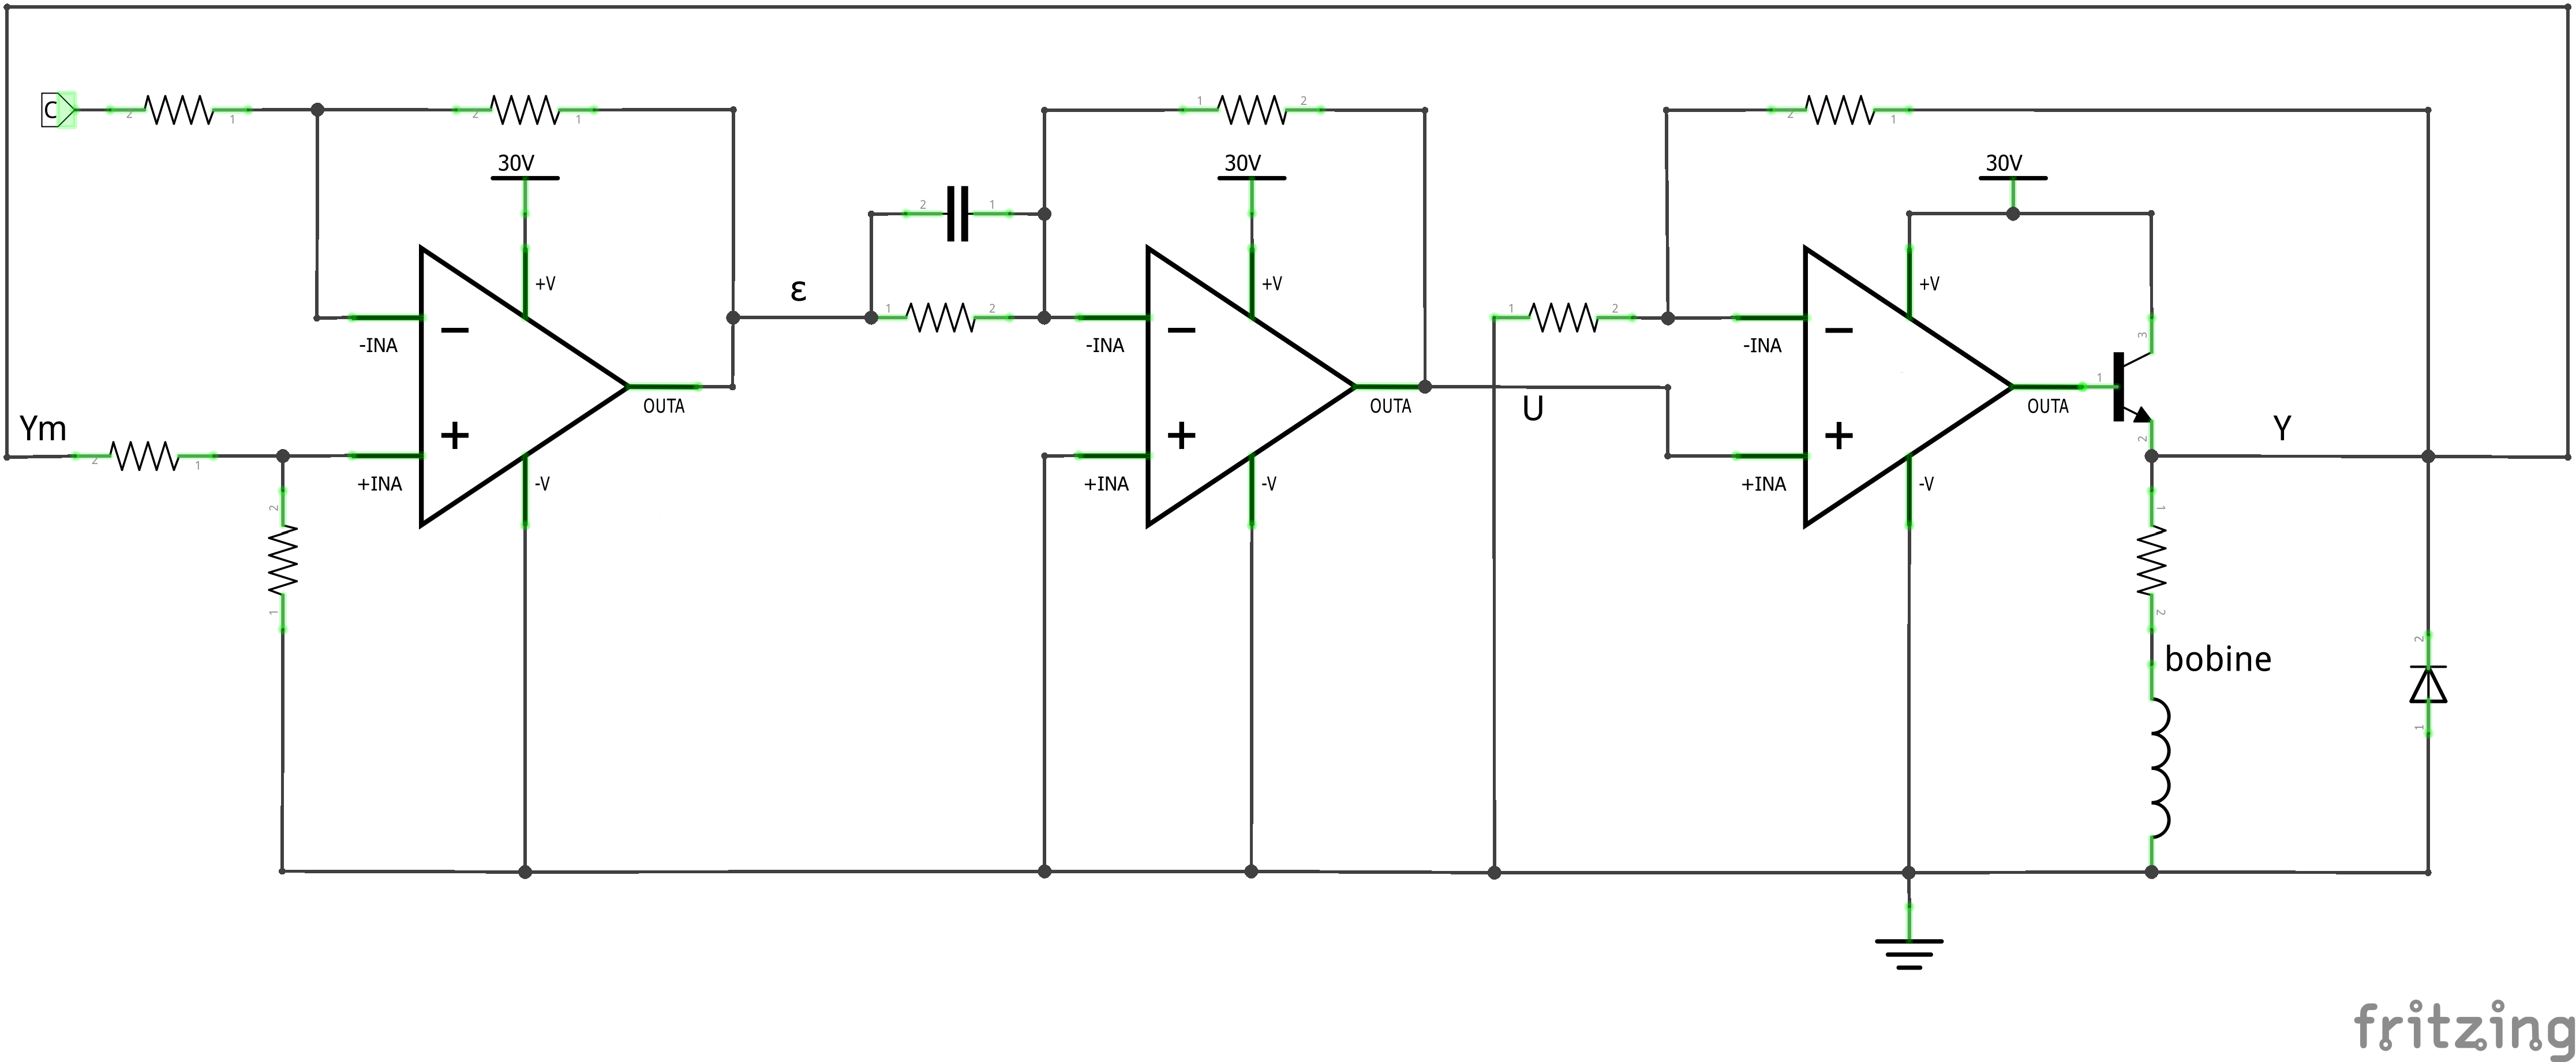
\includegraphics[width=1\textwidth]{Schémas/Modèle complet PD.png} 
\end{center}
\caption{Modélisation complète avec retour (PD)}
\label{fig:Modélisation complète avec retour (PD)}
\end{figure}


\subsection{Conclusions pour cette séance}
On commence à avoir des pistes intéressantes. Les schémas que nous avons réalisés vont nous permettre de se faire une idée du système à concevoir, et nous avons perçu l'importance d'utiliser Matlab pour nous aider dans nos calculs

\section{Travail entre les séance 1 et 2}
\subsection{Correction des éléments de la séance précédente}
Nous avions manqué de temps pour terminer comme nous le souhaitions certains points de la séance précédente. Nous avons travaillé sur les points suivants :
\subsubsection{Matlab}
\textit{Pour plus de détails se référer à la section} \ref{Matlab1}\\

Les schémas avaient étés rendus avec Octave, mais après comparaison des rendus, ceux de Matbab donnent d'autres résultats. Les figures \ref{fig:Bode initial} et \ref{fig:Nyquist initial} ont donc été mises à jour

\subsubsection{Modélisation point par point du système}
\textit{Pour plus de détails se référer à la section} \ref{Modélisation point par point}\\

La figure \ref{fig:Schéma bloc} est maintenant rendue en \LaTeX\\

Pour plus de clarté, les points \ref{Modélisation ampli}, \ref{Modélisation PD} et \ref{Modélisation PID} ont été repris. Les figures \ref{fig:Amplificateur à AOP}, \ref{fig:Régulateur PD} et \ref{fig:Régulateur PID} ont été reprises en \LaTeX. Les figures \ref{fig:Modélisation du bloc amplificateur} et \ref{fig:Modélisation du bloc régulateur (PD)} ont été reprises sur Fritzing, avec un bloc AOP mis à jour\\

Le point \ref{Modélisation complète} a été séparé plus plus de clarté. La figure \ref{fig:Modélisation complète avec retour (PD)} y a été ajoutée

\subsection{Simulation de l'amplificateur}
\begin{multicols}{2}
On veut donc simuler notre bloc amplificateur. Dans l'idéal on devrait avoir le graphique suivant :
\begin{figure} [H]
\begin{center}
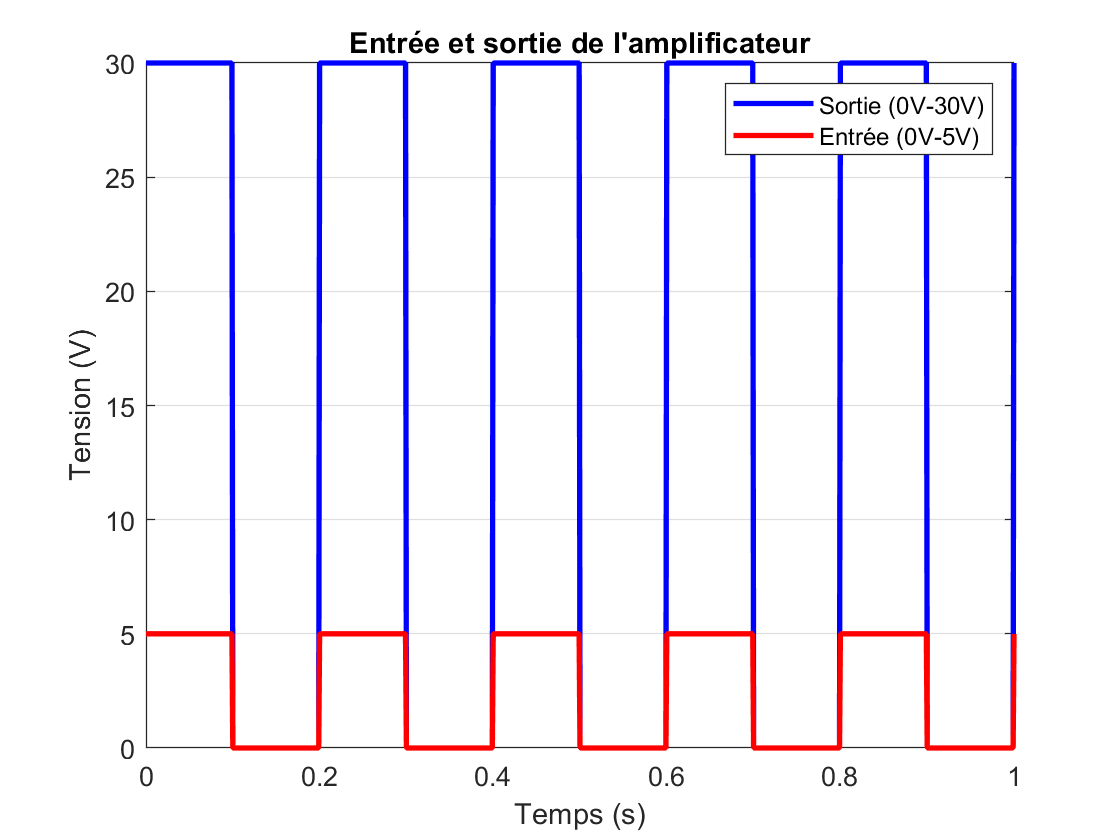
\includegraphics[width=0.5\textwidth]{Schémas/sim matlab ampli.png} 
\end{center}
\caption{Résulat idéal de la simulation}
\end{figure}

On rentre donc le modèle suivant dans LTSPICE :
\begin{figure} [H]
\begin{center}
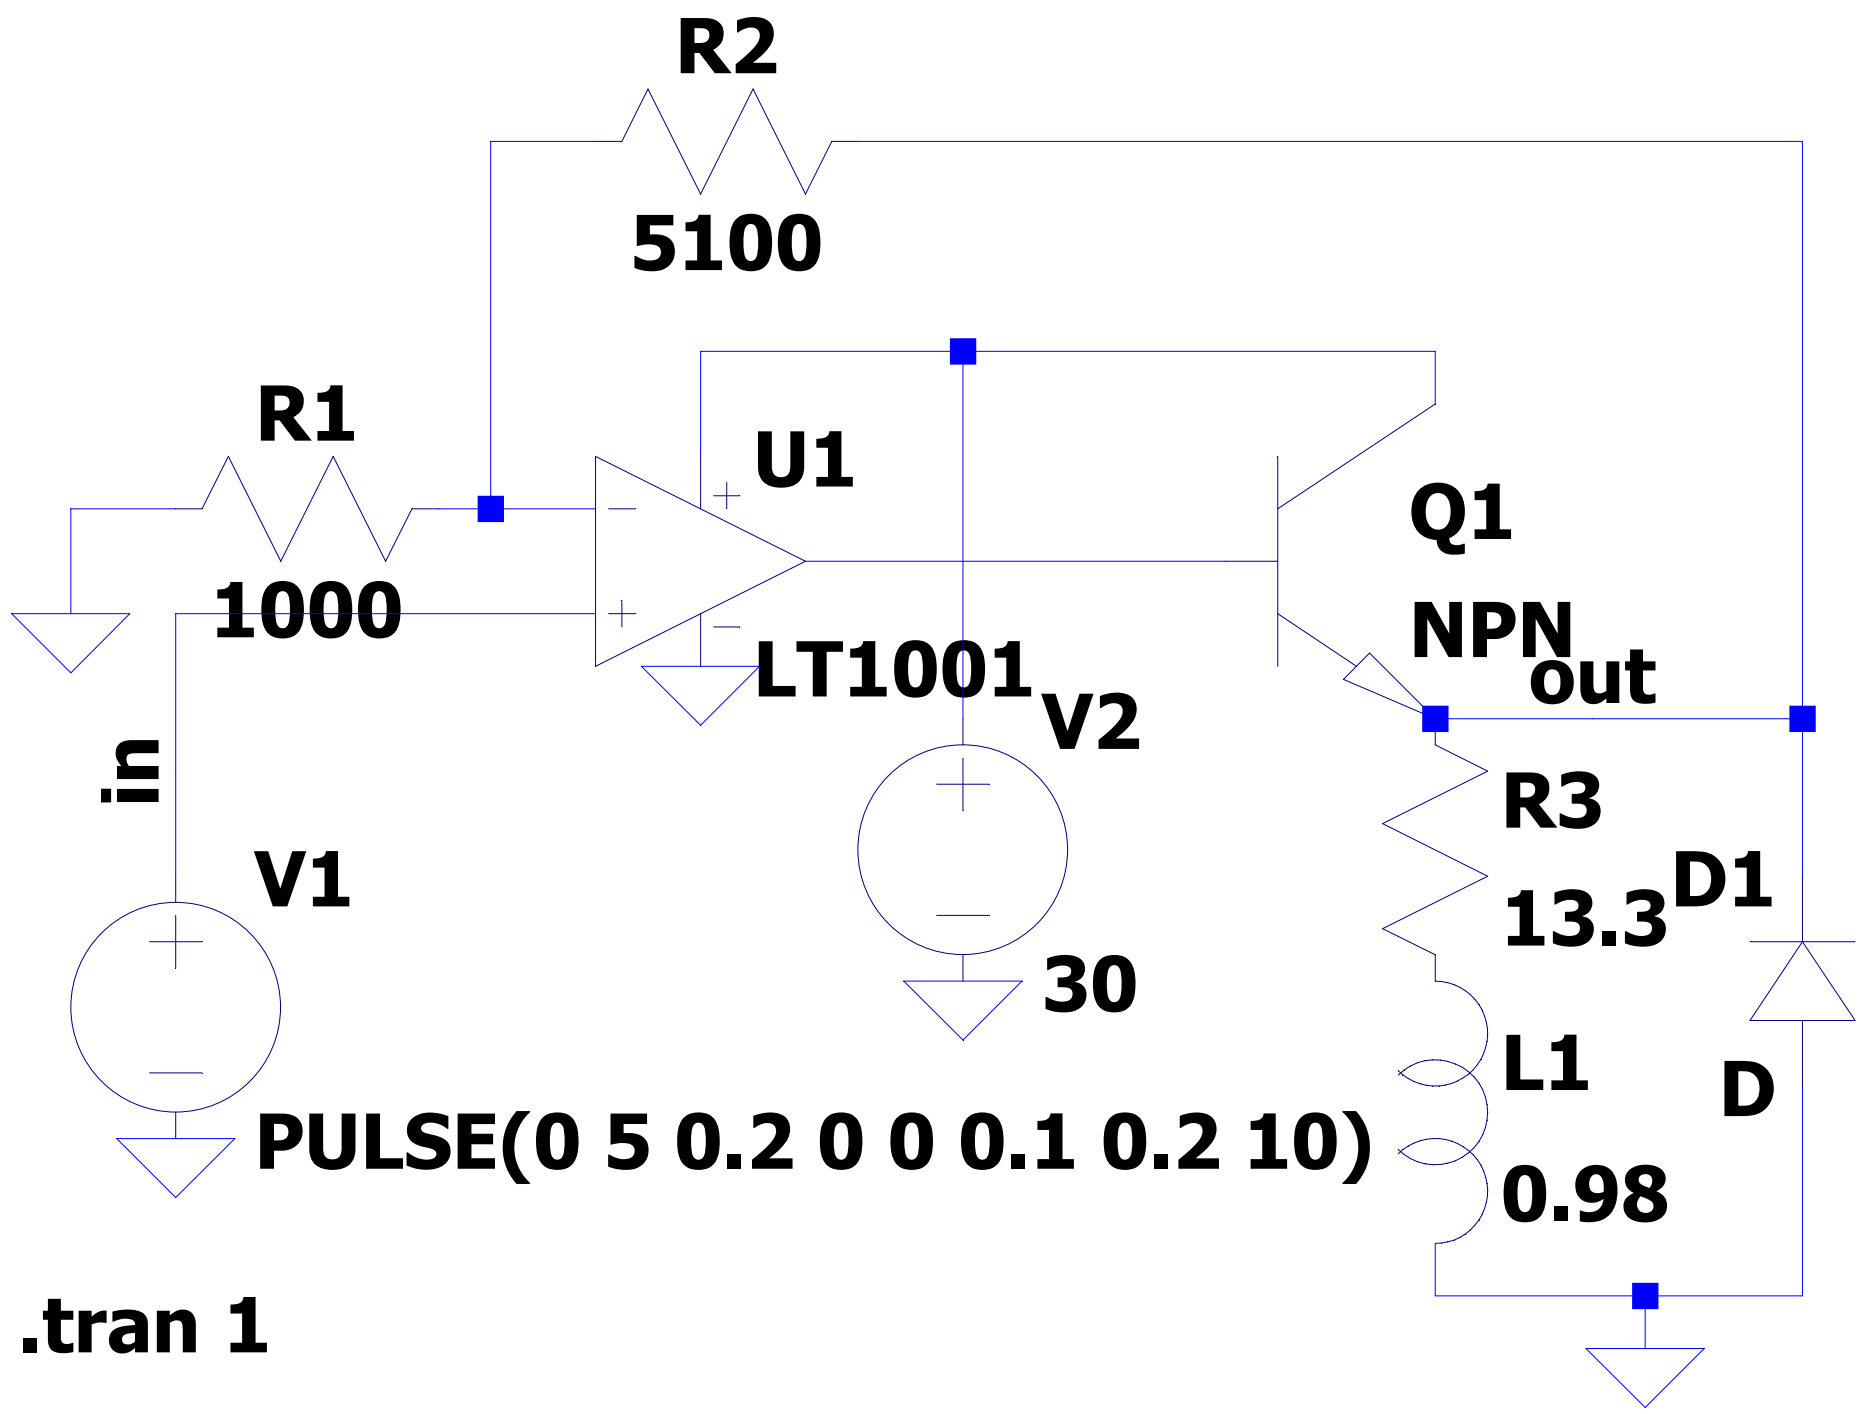
\includegraphics[width=0.5\textwidth]{Schémas/ltspice ampli.png} 
\end{center}
\caption{Schéma LTSPICE de l'amplificateur}
\end{figure}
\label{fig:Simulation ampli}
\end{multicols}

Et on obtient le résultat suivant :
\begin{figure} [H]
\begin{center}
\includegraphics[width=1\textwidth]{Schémas/sim ampli.png} 
\end{center}
\caption{Simulation de l'amplificateur}
\end{figure}

\textbf{Remarques} :
\begin{itemize}
\item On a utilisé un AOP quelconque (le LT1001 en l'occurence)
\item On a utilisé les mesures de la bobine du S1 ($R=13.3\Omega$ et $L=0.98H$)
\item On a utilisé un transistor quelconque
\end{itemize}

On remarque que la simulation correspond au modèle théorique voulu. C'est bon signe pour la suite, il reste à le tester avec des composants réels

\pagebreak
\section{Séance 2 - 18/04/2023}
\subsection{Réflexion sur la numérisation du correcteur}
On va donc chercher à numériser la partie correcteur. Cela correspond aux éléments suivants sur notre schéma bloc :
\begin{figure} [H]
\begin{center}
\begin{tikzpicture}
\sbEntree{E}
\sbSumb{comp}{E}                
\sbRelier[$C$]{E}{comp}
\sbStyleBloc{red,very thick}
\sbBloc{reg}{$R$}{comp}  
\sbRelier[$\varepsilon$]{comp}{reg}
\sbStyleBlocDefaut
\sbBloc{amp}{$A$}{reg}
\sbRelier[$U$]{reg}{amp}
\sbBloc{sys}{$H$}{amp}      
\sbRelier[$X$]{amp}{sys}
\sbSortie{S}{sys}                
\sbRelier[$Y$]{sys}{S}
\sbDecaleNoeudy[4]{S}{U}
\sbStyleBloc{red,very thick}
\sbBlocr{cap}{$B$}{U}        
\sbRelieryx{sys-S}{cap}
\sbRelierxy[$Y_m$]{cap}{comp}
\end{tikzpicture}
\end{center}
\caption{Schéma bloc du système, version électronique numérique}
\end{figure}

On utilisera un STM8s pour la numérisation. On compte utiliser un port analog input pour l'entrée venant du capteur, et un port I/O piloté en PWM pour la sortie $U$

\subsection{Prise en main du STM8s}
On a le brochage du STM8 :
\begin{figure} [H]
\begin{center}
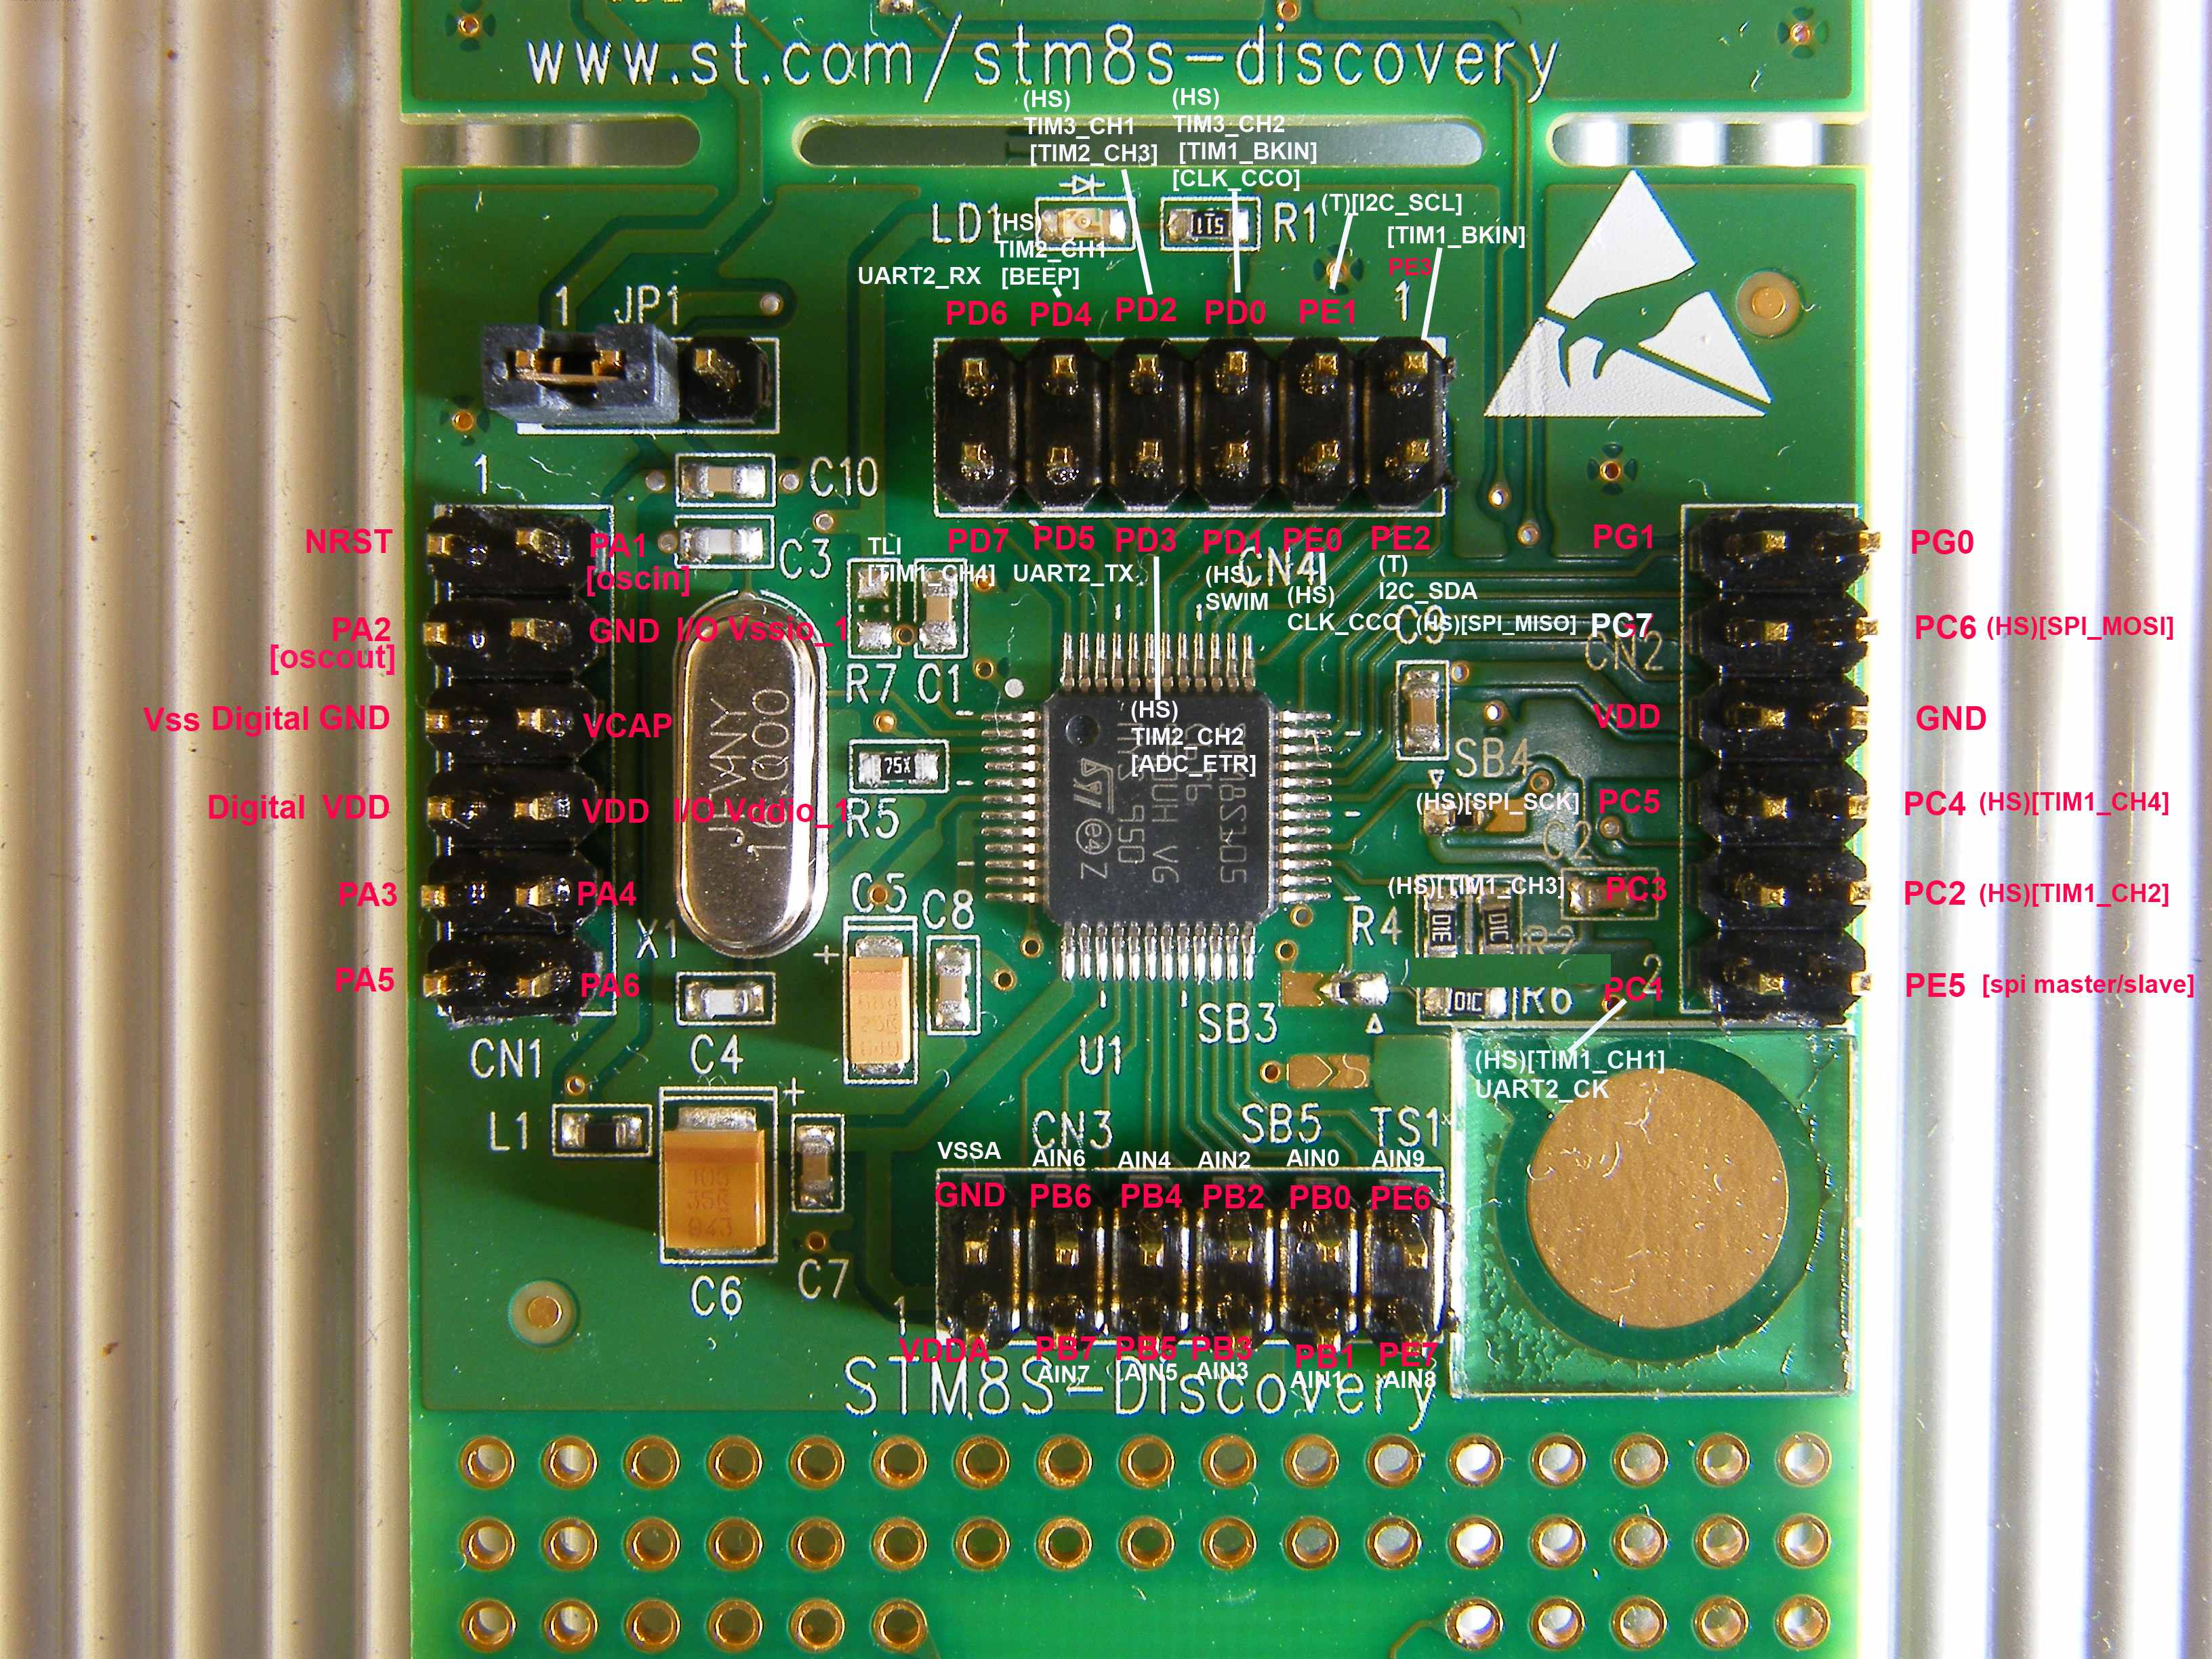
\includegraphics[width=0.6\textwidth]{Schémas/Brochage STM8.jpg} 
\end{center}
\caption{Brochage du STM8s discovery}
\end{figure}

On définit pour le moment qu'on utilise le port $B0$ (Analog 0) pour l'entrée et le port $G0$ pour la sortie (I/O classique)

\subsection{Premier essai de code}
Par la suite, nous avons cherché à faire fonctionner la carte, en vue de pouvoir faire nos mesures. On se base sur l'exemple fourni par ST permettant de faire clignoter la LED installée sur la carte : \href {https://www.st.com/en/embedded-software/stsw-stm8023.html}{\color{blue} fichiers du projet}. Ce projet est écrit en C, compilé à l'aide de Cosmic. On confirme que cela fonctionne

\subsection{Essais avec Arduino}
\medskip
Afin de pouvoir communiquer, notemment via la communication série avec la carte, on a essayé d'installer les librairies nécessaires sur l'Arduino IDE. On se base sur le travail de Michael Mayer pour le site \href {https://circuitdigest.com/microcontroller-projects/programming-stm8s-microcontrollers-using-arduino-ide}{\color{blue} CircuitDigest}. Malgré de nombreuses tentatives, nous n'avons pas réussi à compiler un projet et à l'envoyer sur la carte\\

Sur nos PC, nous obtenons l'erreur suivante :
\begin{lstlisting}
Installing platform sduino:stm8@0.5-pre2
Failed to install platform: sduino:stm8.
Error: 13 INTERNAL: Cannot install platform: installing platform sduino:stm8@0.5-pre2: searching package root dir: no unique root dir in archive, found 'C:\Users\guill\AppData\Local\Arduino15\tmp\package-518500940\STM8S_StdPeriph_Driver' and 'C:\Users\guill\AppData\Local\Arduino15\tmp\package-518500940\cores'
\end{lstlisting}

Et sur les PC de l'école, malgré l'installation des drivers, Arduino ne détecte pas la carte dans la liste des ports disponibles

\subsection{Essais avec STVD}
Nous avons en parallèle repris le code d'un précédent TP, où nous devions implémenter la génération de signaux PWM :
\begin{lstlisting}[language={[x86masm]Assembler}]
stm8/
    #include 'mapping.inc'
    #include 'stm8s105c_s.inc'

    segment 'rom'
debut
    bset PD_DDR,#3
    bset PD_CR1,#3
    bres PD_ODR,#3
    mov TIM4_PSCR,#6
    mov TIM4_ARR,#155
    bset TIM4_IER,#0
    bset TIM4_CR1,#0
    rim
    bset ADC_CR1,#0
    mov ADC_CSR,#$00
    bres ADC_CR2,#3

boucle_infinie
    jra boucle_infinie

    interrupt Timer4_ISR
Timer4_ISR
    bres TIM4_SR,#0
    bcpl PD_ODR,#3
    bset ADC_CR1,#0
attente_fin_conversion
    btjf ADC_CSR,#7,attente_fin_conversion
    bres ADC_CSR,#7
    ld A,#1
    or A,ADC_DRH
    ld TIM4_ARR,A
    iret

    segment 'vectit'
    dc.l {$82000000+debut}
    segment at 8064 'vectit'
    dc.l {$82000000+Timer4_ISR}

    end
\end{lstlisting}

Le but de ce code est de réaliser les actions suivantes :
\begin{itemize}
\item Toutes les 10ms, une interruption se produit et déclenche la conversion ADC, et attend la fin de la conversion
\item La valeur de la conversion est stockée dans le registre TIM4\_ARR, qui est utilisé pour définir la période du timer 4
\end{itemize}
En tant que tel, on peut ensuite utiliser un oscilloscope pour afficher la tension mesurée\\

Nous n'avons pas eu le temps de réfléchir au code, et nous ne savons pas encore si nous préfèrerons le faire en assembleur ou en C

\subsection{Conclusions pour cette séance}
Si nous avons pu prendre en main la carte et réfléchir à l'implémentation du correcteur numériquement, les nombreux freins (problèmes logiciels, logiciels peu ergonomiques...) ont été un frein et nous n'avons pas eu le temps de faire beaucoup de choses. Il sera donc important de travailler entre les deux prochaines séances pour avancer, tant sur la partie analogique, que la partie numérique

\section{Travail entre les séances 2 et 3}
\subsection{Lecture d'une entrée analogique}
Des recherches sur internet nous ont permis de trouver les tutoriels suivants : \href{https://circuitdigest.com/microcontroller-projects/adc-on-stm8s-using-c-compiler-reading-multiple-adc-values-and-displaying-on-lcd}{Tutoriel de CircuitDigest pour ADC} et \href{https://circuitdigest.com/microcontroller-projects/serial-monitor-on-stm8s-using-cosmic-and-stvd}{Tutoriel de CircuitDigest pour la lecture série}. On utilise le code de ces deux tutoriels pour produire le programme suivant :

\begin{lstlisting}[language=C]
#include "STM8S.h"
#include "stm8s103_adc.h"
#include "stm8s103_serial.h"

void main()
{
    // Declarations de variables
    unsigned int ADC_value_1 = 0;
    int ADC_voltage_1 = 0;

    CLK_PeripheralClockConfig(CLK_PERIPHERAL_ADC, ENABLE); // Activer l'horloge peripherique pour l'ADC
    GPIO_Init(GPIOB, GPIO_PIN_0, GPIO_MODE_IN_FL_IT);      // Initialiser le pin PB0 en entree

    Serial_begin(9600);
    Serial_print_string("Bonjour !");
    Serial_newline();
    delay_ms(5000);

    while (1)
    {
        ADC_value_1 = ADC_Read(AIN2);
        ADC_voltage_1 = ADC_value_1 * (2.933); //(3000/1023 =~ 2.933) 
        Serial_print_string("B0: ");
        Serial_print_string(ADC_value_1);
        Serial_print_string(" -> ");
        Serial_print_string(ADC_voltage_1);
        Serial_print_string(" mV");
        Serial_newline();
        delay_ms(500);
    }
}
\end{lstlisting}

On aura donc à priori besoin des fichiers suivants :
\begin{itemize}
\item \href{https://github.com/CircuitDigest/STM8S103F3_SPL}{Fichiers de base} 
\item \href{https://github.com/CircuitDigest/STM8S103F3_SPL/blob/master/stm8s103%20Libraries/stm8s103_Serial.h}{Fichier Serial.h}
\item \href{https://github.com/CircuitDigest/STM8S103F3_SPL/blob/master/inc/stm8s103_ADC.h}{Fichier ADC.h}
\end{itemize}

\subsection{Génération d'un signal PWM}
\subsubsection{Code}
Des recherches sur internet nous ont permis de trouver le tutoriel suivant : \href{https://circuitdigest.com/microcontroller-projects/pulse-width-modulation-pwm-with-stm8-using-cosmic-c-and-stvd}{Tutoriel de CircuitDigest}. On en retire le code suivant :

\begin{lstlisting}[language=C]
#include "STM8S.h"

void delay_ms(int ms)
{
	int i;
	int j;
    for (i = 0; i <= ms; i++)
    	{
        for (j = 0; j < 120; j++) {_asm("nop");}
    }
}

void main(void)
{
    GPIO_DeInit(GPIOD);
    TIM2_DeInit();
    GPIO_Init(GPIOD, GPIO_PIN_4, GPIO_MODE_OUT_PP_HIGH_FAST);
    TIM2_OC1Init(TIM2_OCMODE_PWM1, TIM2_OUTPUTSTATE_ENABLE, 1000, TIM2_OCPOLARITY_HIGH);
    TIM2_TimeBaseInit(TIM2_PRESCALER_1, 500);
    TIM2_Cmd(ENABLE);
    while (TRUE)
    {
        signed int pwm_duty = 500;
        TIM2_SetCompare1(pwm_duty);
    }
}
\end{lstlisting}

\subsubsection{Description du code}
Dans la fonction main, les fonctions de configuration et d'initialisation suivantes sont appelées :
\begin{itemize}
\item \lstinline$GPIO_DeInit(GPIOD)$ : réinitialisation des paramètres du port D
\item \lstinline$TIM2_DeInit()$ : réinitialisation du Timer 2
\item \lstinline${GPIO_Init(GPIOD, GPIO_PIN_4, GPIO_MODE_OUT_PP_HIGH_FAST)$ : configuration de la broche PD4 en sortie push-pull avec une vitesse élevée
\item \lstinline$TIM2_OC1Init(...)$ : configuration du Timer 2 pour générer un signal PWM en mode 1 avec un rapport cyclique initial de 1000 (50\%)
\item \lstinline$TIM2_TimeBaseInit(TIM2_PRESCALER_1, 500)$ : configuration de la base de temps du Timer 2 avec un prédiviseur de 1 et une valeur d'autorechargement de 500
\item \lstinline$TIM2_Cmd(ENABLE)$ : activation du Timer 2
\end{itemize}
\pagebreak
Enfin, la partie :
\begin{lstlisting}[language=C]
while (TRUE)
    {
        signed int pwm_duty = 500;
        TIM2_SetCompare1(pwm_duty);
    }
\end{lstlisting}
Génère un signal PWM de rapport cyclique (\lstinline$pwm_duty$/10)\%

\subsubsection{Fichiers nécessaires}
Comme précedemment, on aura besoin des fichiers des \href{https://github.com/CircuitDigest/STM8S103F3_SPL}{Fichiers de base}

\section{Séance 3 - 03/05/2023}
\subsection{Partie électronique numérique}
\subsubsection{Récupération d'une entrée}
Nous auront donc un capteur renvoyant des valeurs entre $0V$ et $3V$, correspondant à la distance avec la bille, dont il faudra récupérer les valeurs à l'aide d'un port analogique du STM8. Nous souhaitions récupérer les valeurs et les renvoyer vers un port série. Cependant, malgré l'installation de drivers et des bibliothèques nécessaires, que ce soit avec le moniteur Arduino ou avec Putty, nous n'avons pas réussi à récupérer les valeurs renvoyées par la carte. Le code que nous avions écrit plus haut compile cependant, et la carte arrive à l'exécuter. Nous pourrons vérifier son fonctionnement lorsque nous auront réussi à générer des signaux PWM.

\subsubsection{Génération de signaux PWM}
Nous avons donc tenté de générer des signaux PWM en utilisant notre code. Lorsque le programme est exécuté, on constate bien une tension entre PD4 et la masse, mais cette tension est constante. Nous avons tenté de nombreuses modifications sans succès. Nous avons donc voulu essayer des exemples présents en ligne, afin d'au moins se faire une idée sur la faisabilité de la génération de ces signaux.\\
\medskip
Voici une liste des sites que nous avons utilisé, ainsi que le résultat que nous avons pu obtenir au final :
\begin{itemize}
\item \href{https://www.st.com/en/embedded-software/stsw-stm8036.html}{Site de ST Microelectronics} : ne contient pas un programme complet, ne compile pas, pas de résultats concluants
\item \href{https://circuitdigest.com/microcontroller-projects/pulse-width-modulation-pwm-with-stm8-using-cosmic-c-and-stvd}{Site de CircuitDigest} : code dont nous nous étions inspiré, génère une tension positive constante mais pas de PWM
\item \href{https://blog.mark-stevens.co.uk/2012/08/generating-pwm-signals-using-the-stm8s/}{Site de Mark-Stevens} : ne contient pas les fichiers nécessaire à la compilation, pas de résultats concluants
\item \href{https://embedded-lab.com/blog/starting-stm8-microcontrollers/20/}{Site d'Embedded lab} : compile avec quelques modifications, mais pas de tension en sortie des ports de la carte
\item \href{https://gist.github.com/stecman/f748abea0332be1e41640fd25b5ca861}{Github de stecman} : nous n'avons pas eu le temps de regarder, mais semble intéressant
\end{itemize}
Au final nous n'avons pas encore de résultats. Il faudra par la suite soit trouver pourquoi nous n'arrivons pas à générer ces signaux avec un programme en C, soit essayer en assembleur. Le problème de l'assembleur est qu'il sera probablement plus difficile d'implémenter nos calculs de PID.

\subsubsection{Brouillon pour un régulateur P}
En parallèle, nous avons commencé à réfléchir à un programme permettant de récupérer l'entrée, d'appliquer un calcul (ici $Kp=1$), et de produire une sortie avec un signal PWM. Ce code n'a pas encore été testé.

\pagebreak
\begin{lstlisting}[language = C]
#include "stm8s.h"
#include "stm8s_adc1.h"
#include "stm8s_tim1.h"

// Parametre du regulateur proportionnel
#define KP 1.0

// Variables globales
volatile uint16_t consigne = 0;
volatile uint16_t adc_value = 0;

void main(void) {
    // Initialisation des peripheriques (ADC, TIM1, etc.)
    System_Init();

    while (1) {
        adc_value = ADC1_GetConversionValue(); // Lecture de la valeur ADC
        regulation_P(); // Appel de la fonction de regulation proportionnelle
    }
}

void System_Init() {
    // Configuration ADC
    ADC1_Init(ADC1_CONVERSIONMODE_SINGLE, ADC1_CHANNEL_0, ADC1_PRESSEL_FCPU_D2, ADC1_EXTTRIG_TIM, DISABLE, ADC1_ALIGN_RIGHT, ADC1_SCHMITTTRIG_CHANNEL0, DISABLE);
    ADC1_StartConversion();

    // Configuration TIM1 pour PWM
    TIM1_TimeBaseInit(0xFFFF, TIM1_COUNTERMODE_UP, 0, 0);
    TIM1_OC1Init(TIM1_OCMODE_PWM1, TIM1_OUTPUTSTATE_ENABLE, 0, TIM1_OCPOLARITY_HIGH);
    TIM1_Cmd(ENABLE);
    TIM1_CtrlPWMOutputs(ENABLE);

    // Configuration du GPIO pour la sortie PWM
    GPIO_Init(GPIOB, GPIO_PIN_0, GPIO_MODE_OUT_PP_HIGH_FAST);

    // Configuration du GPIO pour l'entree analogique (ADC)
    GPIO_Init(GPIOA, GPIO_PIN_0, GPIO_MODE_IN_FL_NO_IT);
}

// Fonction de mise a jour de la consigne
void set_consigne(uint16_t value) {
    consigne = value;
}

// Fonction de regulation proportionnelle
void regulation_P() {
    float erreur = (float)consigne - (float)adc_value;
    float sortie = KP * erreur;

    // Limiter la sortie entre 0 et la valeur maximale du compteur (ici 0xFFFF)
    if (sortie < 0) {
        sortie = 0;
    } else if (sortie > 0xFFFF) {
        sortie = 0xFFFF;
    }

    // Mise a jour de la sortie PWM
    TIM1_SetCompare1((uint16_t)sortie);
}
\end{lstlisting}

\subsection{Partie électronique analogique}
\subsubsection{Matériel utilisé}
On utilise la bobine n°5\\
On utilise la boule "38" pesant $37.6g$ et mesurant $49.74mm$ de diamètre

\subsubsection{Calcul du point de fonctionnement}
On commence par relier la bobine à l'alim :
\begin{figure}[H]
\centering
\begin{circuitikz}
\draw
(0,0)
to[V, l=$28\text{V}$] (0,3)
-- (2,3)
to[R, l=$R$, -] (2,1.5)
to[cute inductor, l=$L$, -] (2,0)
-- (0,0);
\draw [dashed] (1.4,3.1) rectangle (2.6,-0.1) node at (2,0) [below] {Bobine};
\end{circuitikz}
\caption{Bobine alimentée}
\end{figure}

On a donc $V=28V$, et on souhaite mesurer $I$ en fonction $z$ (distance entre le bas de la bobine et le centre de la boule)\\

\begin{multicols}{2}
On relève les valeurs suivantes :\\\\
\begin{tabular}{|c|c|c|}
\hline 
\textbf{Hauteur $z$} & \textbf{Courant $I$}\\ 
\hline 
$0.0330m$ & $0.542A$ \\ 
\hline 
$0.0375m$ & $0.702A$ \\ 
\hline 
$0.0434m$ & $0.922A$ \\ 
\hline 
$0.0462m$ & $1.112A$ \\ 
\hline 
$0.0527m$ & $1.342A$ \\ 
\hline 
$0.0555m$ & $1.431A$ \\ 
\hline 
$0.0588m$ & $1.601A$ \\ 
\hline 
$0.0613m$ & $1.822A$ \\ 
\hline 
$0.0623m$ & $1.851A$ \\ 
\hline 
$0.0626m$ & $1.952A$ \\ 
\hline
\end{tabular} \\

On souhaite obtenir une interpolation affine de ces valeurs. On rentre dans MATLAB la commande \lstinline$polyfit(z,I,1);$ et on obtient que :\\

$\boxed{I=45.8215z-1.0243}$\\

\columnbreak
On produit donc la courbe suivante :
\begin{figure}[H]
\begin{center}
\begin{tikzpicture}
\begin{axis}[
xlabel=Hauteur $z$ (m),
ylabel=Courant $I$ (A),
xmin=0.033, xmax=0.0626,
ymin=0, ymax=2,
xtick={0.035,0.04,0.045,0.05,0.055,0.06},
ytick={0,0.5,1,1.5,2},
legend pos=north west,
legend style={font=\tiny},
ymajorgrids=true,
grid style=dashed,
]
\addplot[color=blue, mark=square]
coordinates {(0.033,0.542)(0.0375,0.702)(0.0434,0.922)(0.0462,1.112)(0.0527,1.342)(0.0555,1.431)(0.0588,1.601)(0.0613,1.822)(0.0623,1.851)(0.0626,1.952)};
\legend{Intensité mesurée}
\addplot[color=red,domain=0.033:0.0623] {45.8215*x-1.0243};
\addlegendentry{Interpolation affine}
\end{axis}
\end{tikzpicture}
\caption{Courbe de l'intensité mesurée en fonction de la distance}
\end{center}
\end{figure}

\end{multicols}

Au final, on choisit $I_0=1.3A$, ce qui nous donne $z_0=5.1cm$

\pagebreak
\subsubsection{Résistance de la bobine}
On réalise le montage suivant :
\begin{figure}[H]
\centering
\begin{circuitikz}
\draw
(0,0) to[V, l=$28\text{V}$] (0,5) -- (2,5)
to[rmeterwa, t=A, i=$i$] (2,3)
to[R, l=$R$, -] (2,1.5)
to[cute inductor, l=$L$, -] (2,0)
-- (0,0);
\draw [dashed] (1.4,3.1) rectangle (2.6,-0.1) node at (2,0) [below] {Bobine};
\draw (2,0) -- (4,0) to[rmeterwa, t=V] (4,3) -- (2,3);
\end{circuitikz}
\caption{Mesure de la résistance}
\end{figure}

Après avoir patienté un moment, pour laisser le temps aux caractéristiques de la bobine d'être stables, on mesure $U=27.57V$ et $I=1.95A$\\
On obtient donc la résistance de la bobine $\boxed{R=14.1\Omega}$

\subsubsection{Inductance de la bobine}
On réalise le montage suivant :
\begin{figure}[H]
\centering
\begin{circuitikz}
\draw
(0,0) to[sinusoidal voltage source, l=$2\text{V}$, f=1Hz] (0,4) -- (2,4)
to [iloop, name=I] (2,3)
to[R, l=$R$, -] (2,1.5)
to[cute inductor, l=$L$, -] (2,0)
-- (0,0);
\draw [dashed] (1.4,3.1) rectangle (2.6,-0.1) node at (2,0) [below] {Bobine};
\draw (2.4,3.5) -- ++(1.5,0)
to[oscope] ++(0,-2) node[ground]{};
\end{circuitikz}
\caption{Mesure de l'inductance}
\end{figure}

Après avoir patienté un moment, pour laisser le temps aux caractéristiques de la bobine d'être stables, on mesure un déphase $\varphi=150$°

\begin{figure} [H]
\begin{center}
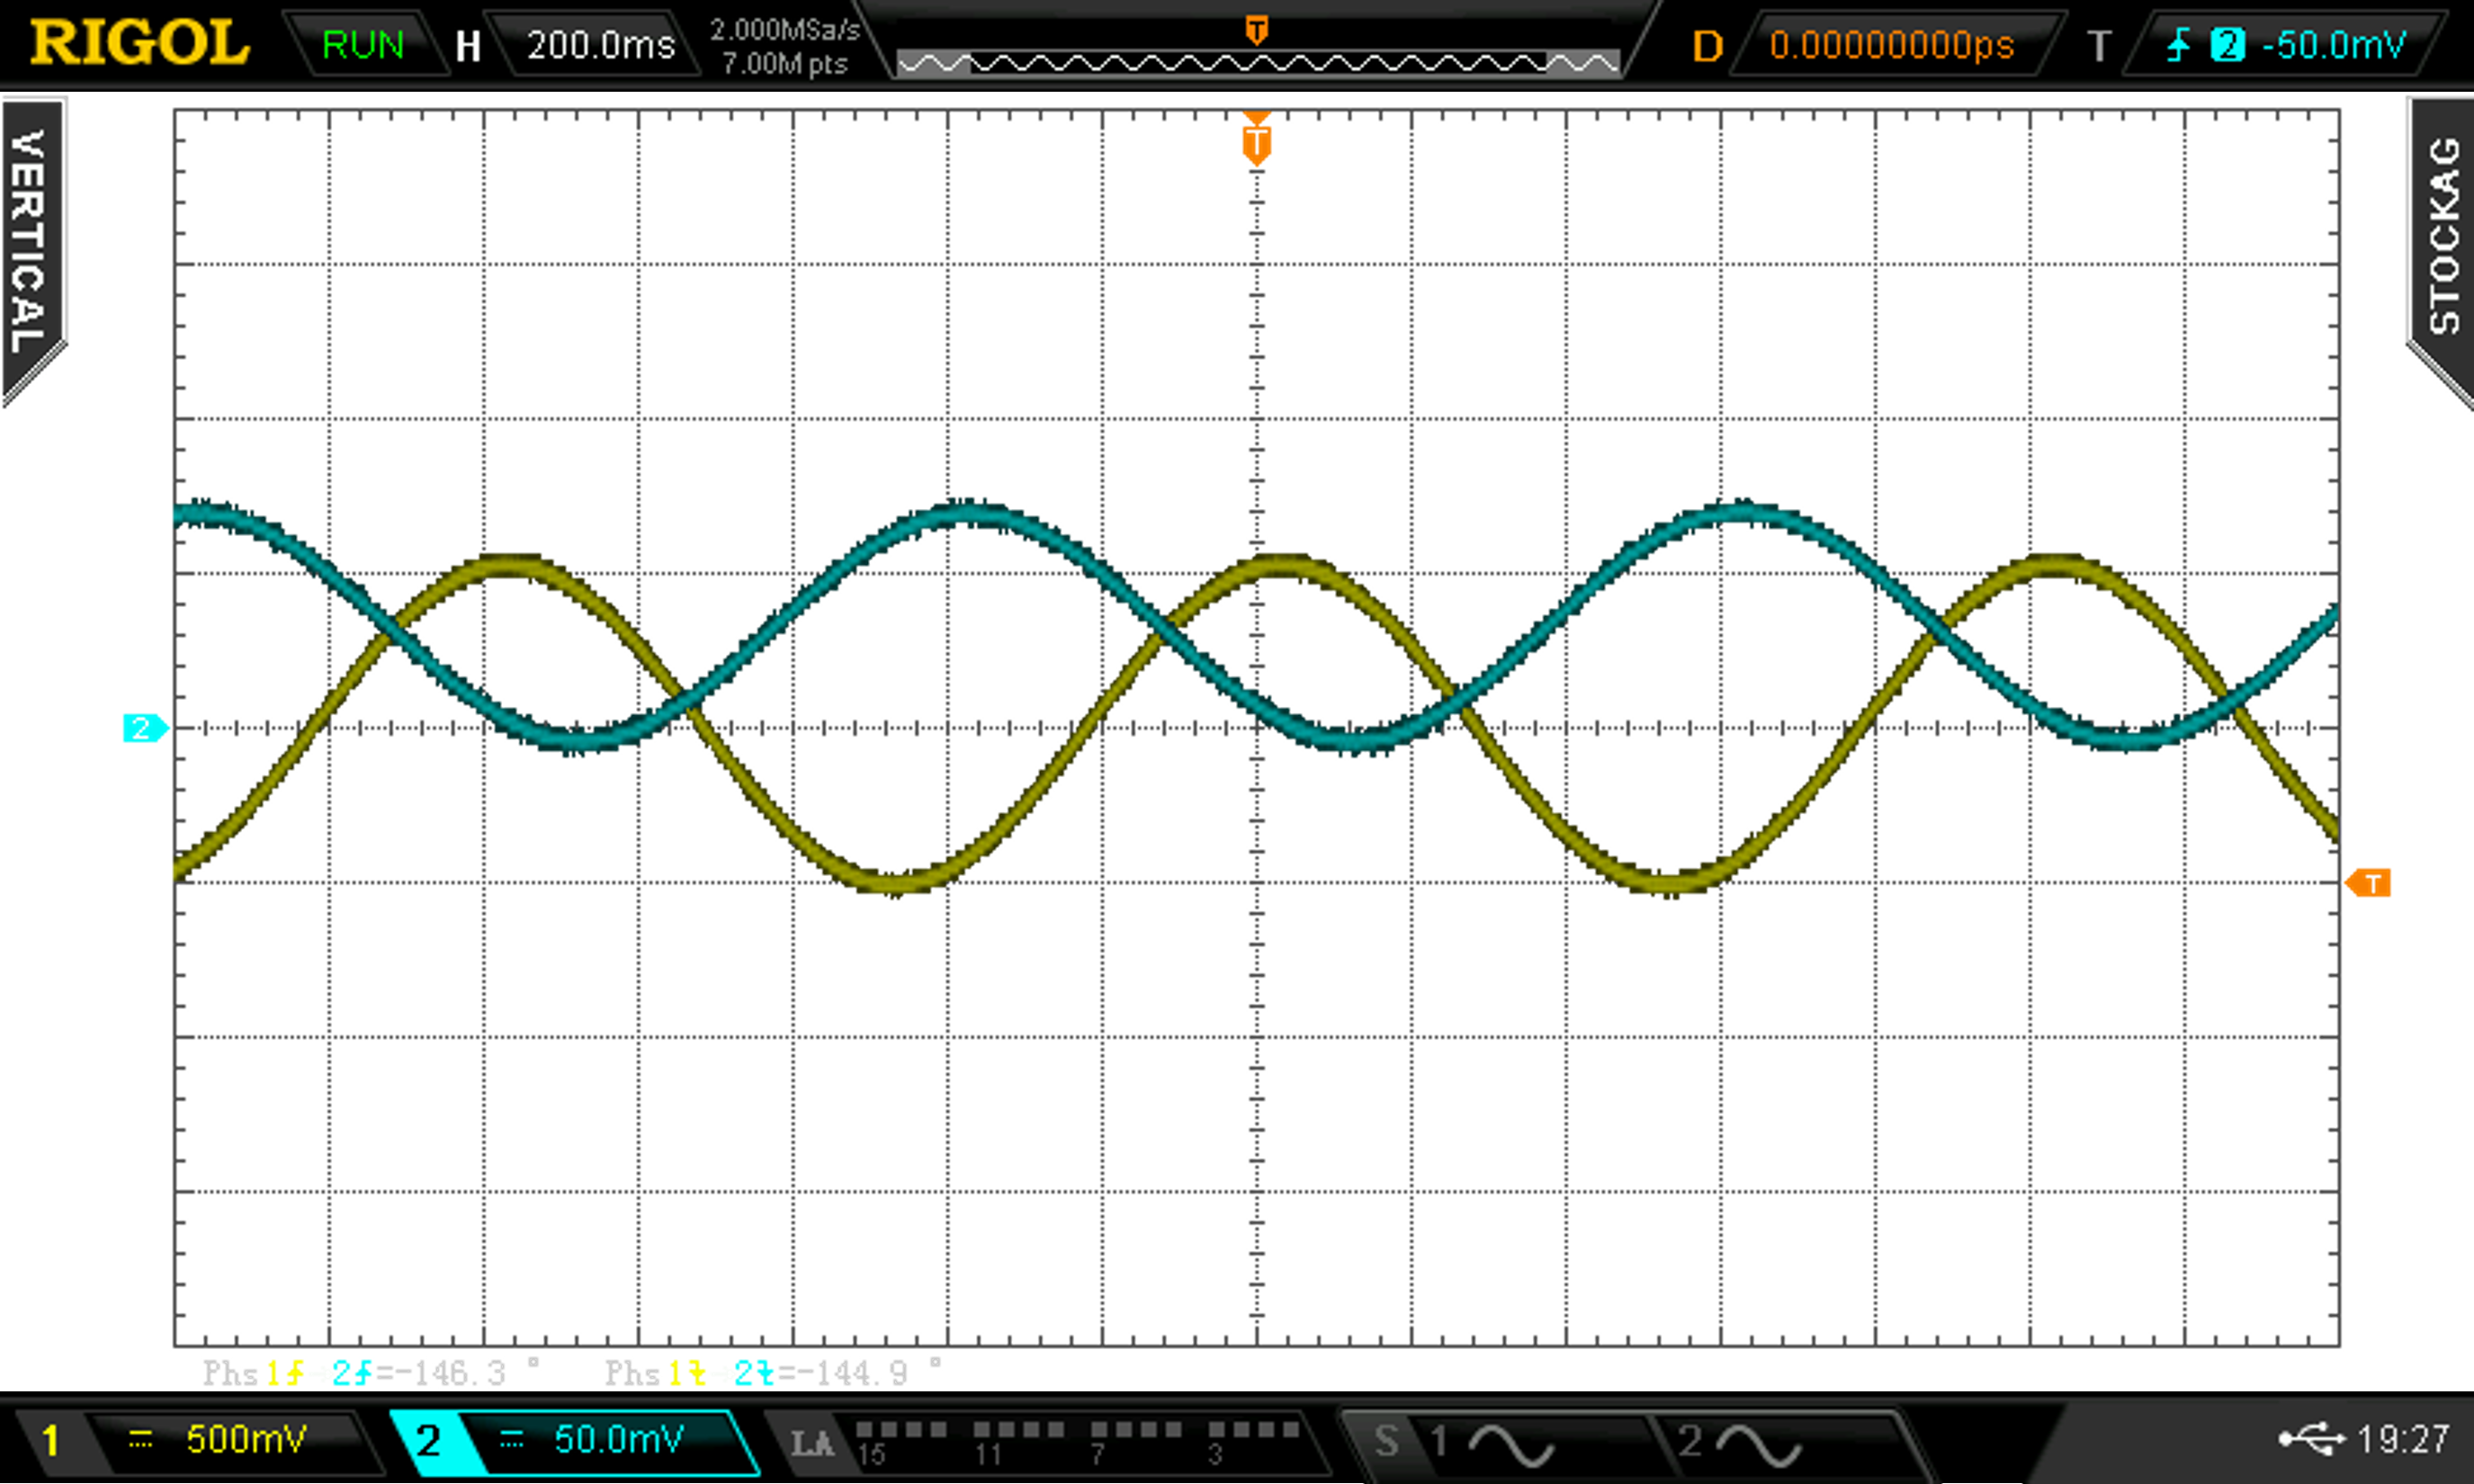
\includegraphics[width=0.5\textwidth]{Schémas/Mesure inductance bobine.png} 
\end{center}
\caption{Réponse de la bobine}
\end{figure}

On calcule donc que l'inductance de la bobine vaut $-\dfrac{R\cdot \tan \varphi}{2\pi f} = -\dfrac{14.1\cdot \tan 150}{2\pi}\boxed{=1.296H}$

\subsection{Conclusions}
Si nous avons peu avancé sur la partie numérique, nous avons pu caractériser la bobine, ce qui nous servira pour la suite dans la modélisation précise de notre système

\section{Séance 4 - 02/06/2023}
Lors de cette séance, nous nous sommes donnés l'objectif de réaliser l'ampli sur platine d'essai, afin de confirmer notre simulation

\subsection{Choix des composants}
\begin{itemize}
\item Transistor : TIP122
\item AOP : TL081
\item Diode : 1N4007
\end{itemize}

\subsection{Réalisation}
Nous avons réalisé le montage présenté dans la partie \ref{fig:Simulation ampli}. Pour le moment le meilleur résultat que nous ayons obtenu est le suivant :

\begin{figure} [H]
\begin{center}
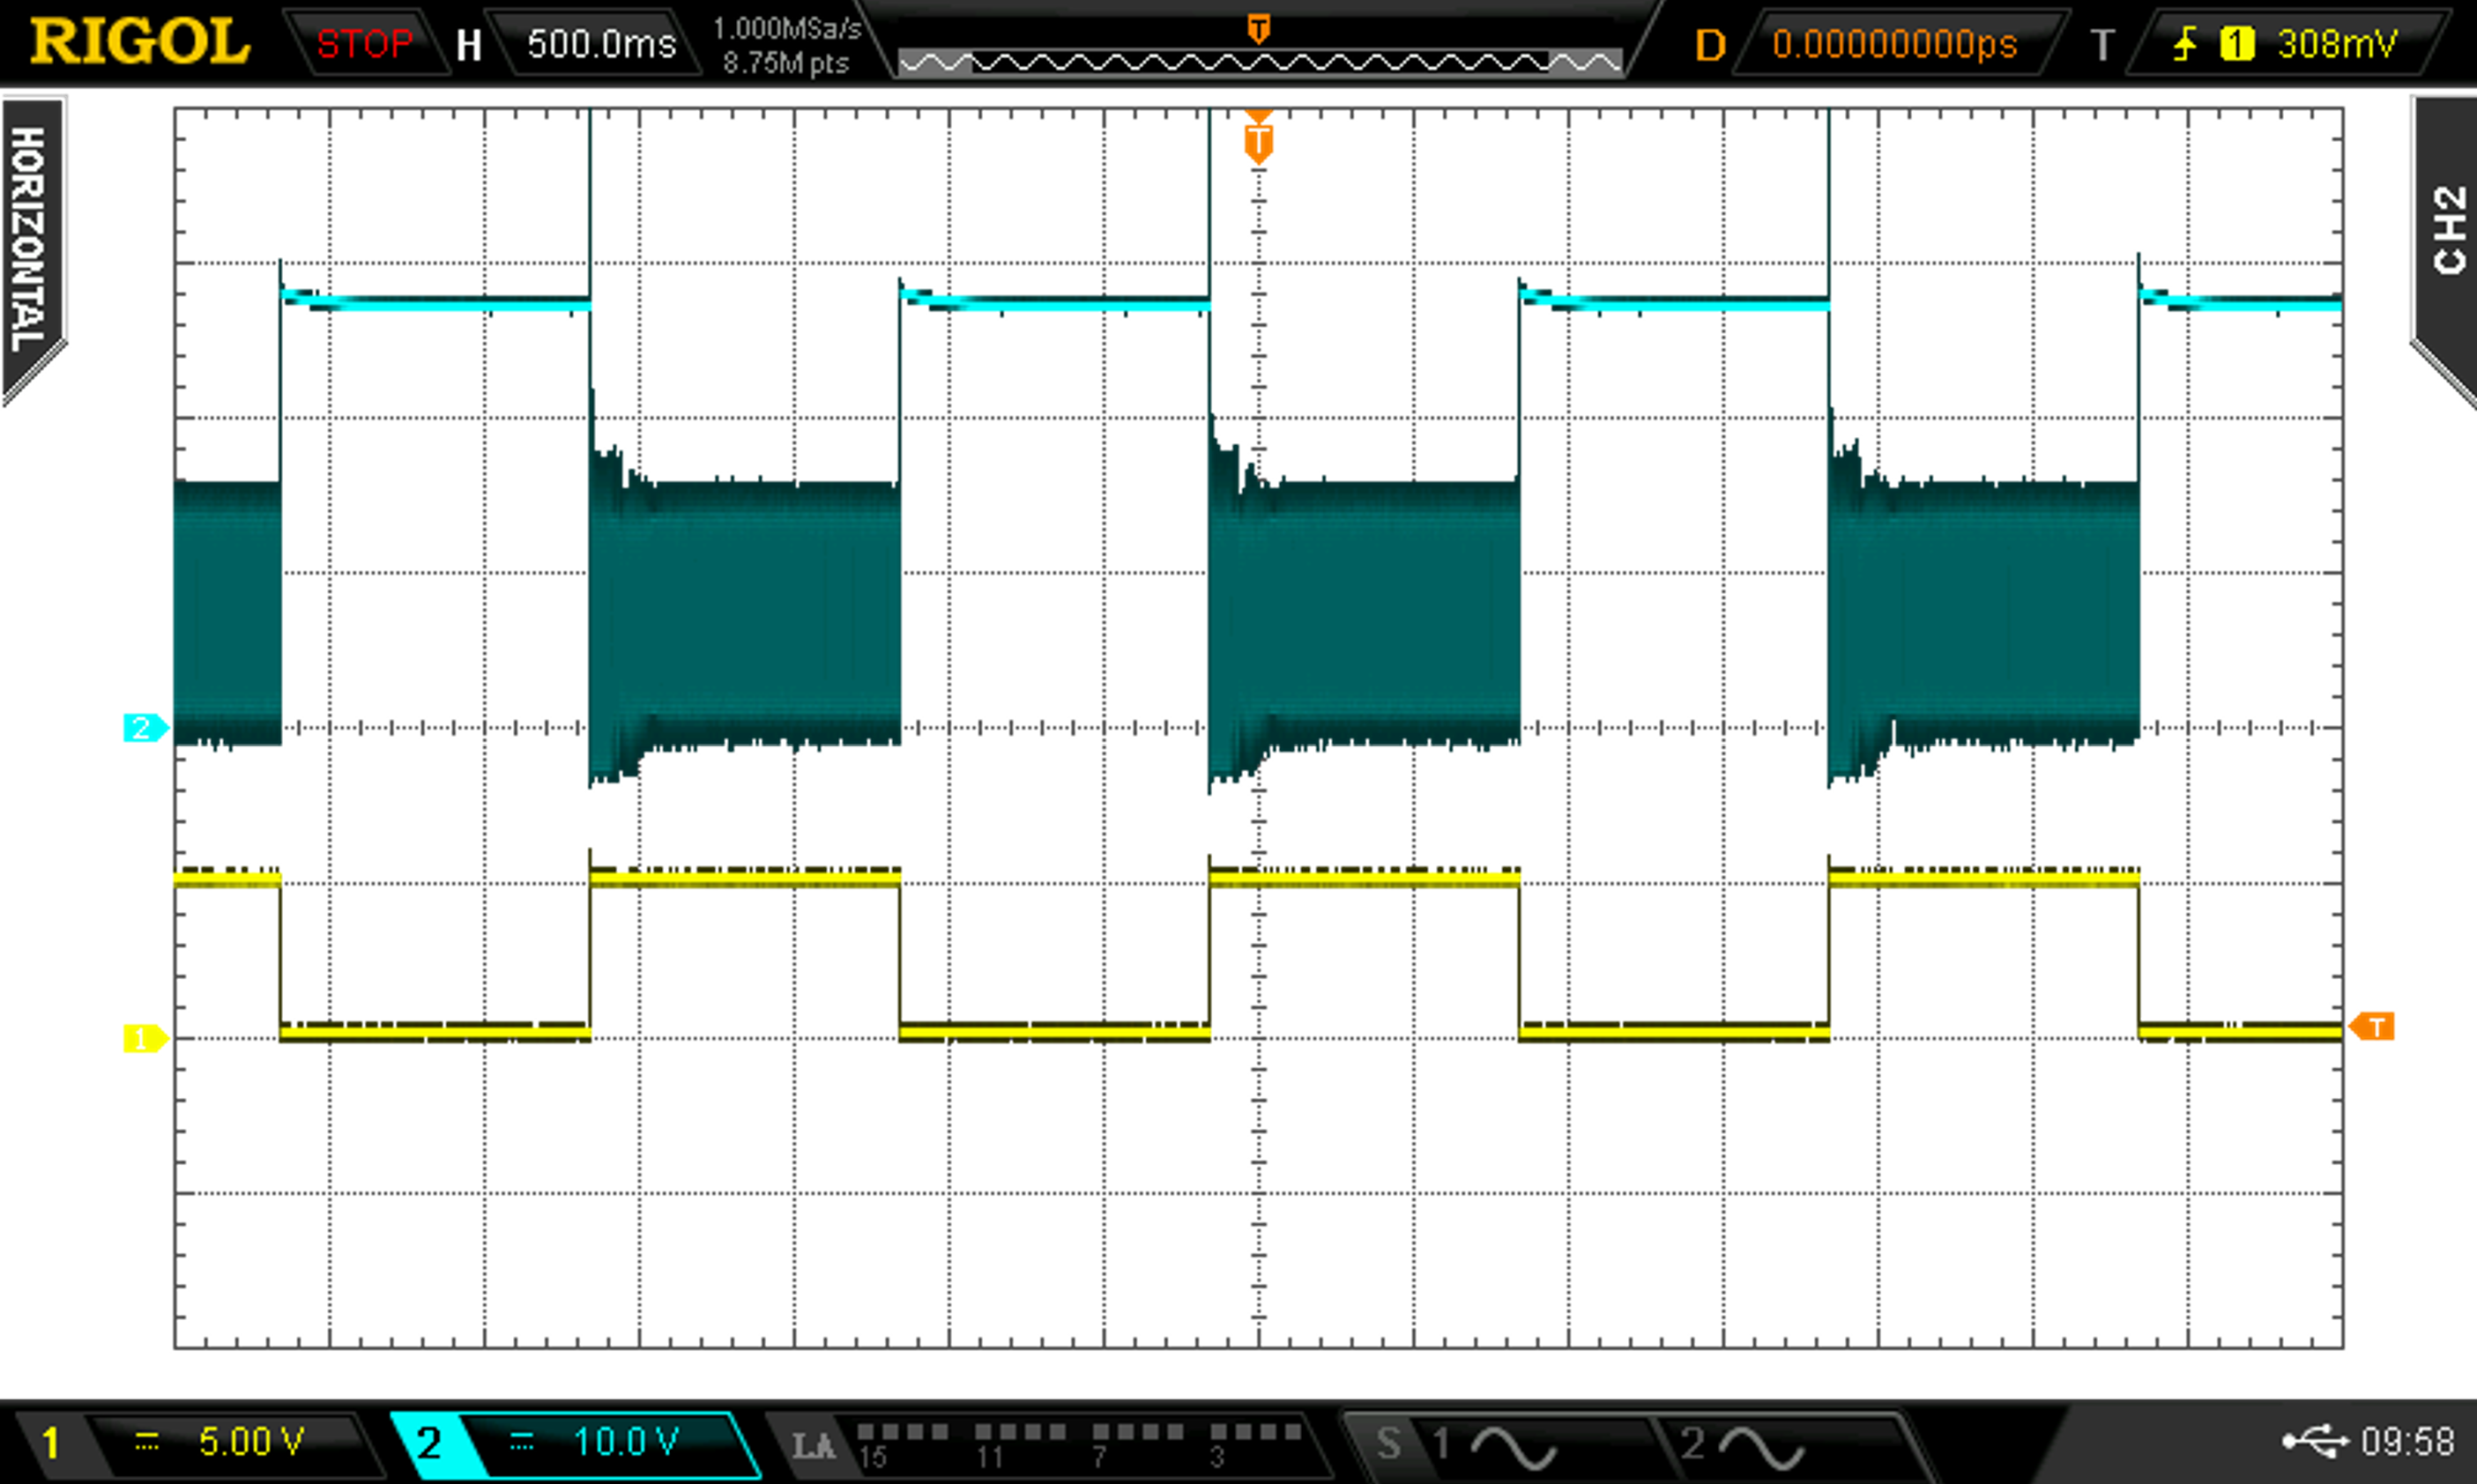
\includegraphics[width=1\textwidth]{Schémas/Mesure ampli TL.png} 
\end{center}
\caption{Mesure du montage amplificateur}
\end{figure}

On a en jaune la commande et en bleu la sortie. Au final, on sent bien que la bille est plus ou moins attirée, mais nous n'avons pas l'effet "on-off" que nous souhaitions obtenir.
Un autre problème auquel nous avons été confronté est que le courant délivré par le montage est beaucoup trop faible : entre 0.1A et 0.4A alors qu'avec la distance qu'on avait mise pour tester le montage, la bille ne pouvait décoller qu'à partir d'environ 1,6A

\subsection{Pistes pour la suite}
Il semblerait que le TL081 ne soit pas adapté à notre montage. On essaiera à la prochaine séance d'utiliser un LM342 à la place

\pagebreak
\section{Bibliographie}
Liste des sites utilisés pour la réalisation du projet :
\begin{itemize}
\item \href{https://www.overleaf.com/learn}{Overleaf, guide d'utilisation du \LaTeX{}}
\item \href{https://chat.openai.com/chat}{ChatGPT, modèle de langage automatisé}
\item \href{https://ctan.mines-albi.fr/graphics/pgf/contrib/circuitikz/doc/circuitikzmanual.pdf}{Manuel de Circuitikz}
\item \href{https://sciences-indus-cpge.papanicola.info/IMG/pdf/schemabloc.pdf}{Manuel des Schéma-blocs avec PGF/TIKZ}
\item \href{https://sciences-indus-cpge.papanicola.info/IMG/pdf/schemabloc.pdf}{Manuel des Schéma-blocs avec PGF/TIKZ}
\item \href{https://circuitdigest.com/microcontroller-projects/getting-started-with-stm8s-using-stvd-and-cosmic-c-compiler}{Tutoriels de CircuitDigest pour STM8s}
\end{itemize}

\end{document}